% zip files.zip ms63.tex CMD_cuts_double.pdf main_figure.pdf gap.pdf vb_vs_teff.pdf vb_vz.pdf field_comparison.pdf bib.bib ms.pdf

\documentclass{aastex63}

% Latin
\newcommand{\ie}{{\it i.e.}}
\newcommand{\eg}{{\it e.g.}}
\newcommand{\etal}{{\it et al.}}

% Missions & Spacecraft
\newcommand{\kepler}{{Kepler}}
\newcommand{\Kepler}{{Kepler}}
\newcommand{\corot}{{\it CoRoT}}
\newcommand{\Ktwo}{{\it K2}}
\newcommand{\ktwo}{\Ktwo}
\newcommand{\TESS}{{\it TESS}}
\newcommand{\tess}{{\it TESS}}
\newcommand{\LSST}{{\it LSST}}
\newcommand{\lsst}{{\it LSST}}
\newcommand{\Wfirst}{{\it WFIRST}}
\newcommand{\wfirst}{{\it WFIRST}}
\newcommand{\SDSS}{{\it SDSS}}
\newcommand{\PLATO}{{\it PLATO}}
\newcommand{\plato}{{\it PLATO}}
\newcommand{\Gaia}{{\it Gaia}}
\newcommand{\gaia}{{\it Gaia}}
\newcommand{\panstarrs}{{\it PanSTARRS}}
\newcommand{\LAMOST}{{\it LAMOST}}
\newcommand{\lamost}{{\it LAMOST}}

% Units and Quantities
\newcommand{\Teff}{$T_{\mathrm{eff}}$}
\newcommand{\teff}{$T_{\mathrm{eff}}$}
\newcommand{\FeH}{[Fe/H]}
\newcommand{\feh}{[Fe/H]}
\newcommand{\prot}{$P_{\mathrm{rot}}$}
\newcommand{\pmega}{$\bar{\omega}$}
\newcommand{\logg}{log(g)}
\newcommand{\dnu}{$\Delta \nu$}
\newcommand{\numax}{$\nu_{\mathrm{max}}$}
\newcommand{\degrees}{$^\circ$}
\newcommand{\vx}{$v_{\bf x}$}
\newcommand{\vy}{$v_{\bf y}$}
\newcommand{\vz}{$v_{\bf z}$}
\newcommand{\vb}{$v_{\bf b}$}
\newcommand{\x}{${\bf x}$}
\newcommand{\y}{${\bf y}$}
\newcommand{\z}{${\bf z}$}
\newcommand{\kms}{kms$^{-1}$}
\newcommand{\sigmavb}{$\sigma_{v{\bf b}}$}
\newcommand{\sigmavz}{$\sigma_{v{\bf z}}$}
\newcommand{\mura}{$\mu_\alpha$}
\newcommand{\pmra}{$\mu_\alpha$}
\newcommand{\mudec}{$\mu_\delta$}
\newcommand{\pmdec}{$\mu_\delta$}
\newcommand{\parallax}{$\pi$}
\newcommand{\ra}{$\alpha$}
\newcommand{\dec}{$\delta$}

% Paper-specific and other
\newcommand{\logp}{$\log(P_\mathrm{rot})$}
\newcommand{\gcolor}{$G_{BP} - G_{RP}$}
\newcommand{\mcp}{\citep{mcquillan2014}}
\newcommand{\mct}{\citet{mcquillan2014}}
\newcommand{\sant}{\citet{santos2019}}
\newcommand{\bvector}{${\bf b}$}
\newcommand{\python}{{\it Python}}
\newcommand{\racomment}[1]{{\color{blue}#1}}

% \shorttitle{Calibrating gyrochronology with kinematics}
% \shortauthors{Angus \etal}

\begin{document}

\title{Calibrating gyrochronology using Galactic kinematics}

% \correspondingauthor{Ruth Angus}
% \email{rangus@amnh.org}

\author{Ruth Angus}
\affiliation{Department of Astrophysics, American Museum of Natural History,
200 Central Park West, Manhattan, NY, USA}
\affiliation{Center for Computational Astrophysics, Flatiron Institute,
162 5th Avenue, Manhattan, NY, USA}
\affiliation{Department of Astronomy, Columbia University, Manhattan, NY, USA}

\author{Yuxi (Lucy) Lu}
\affiliation{Department of Astronomy, Columbia University, Manhattan, NY, USA}
\affiliation{Department of Astrophysics, American Museum of Natural History,
200 Central Park West, Manhattan, NY, USA}

\author{Dan Foreman-Mackey}
\affiliation{Center for Computational Astrophysics, Flatiron Institute,
162 5th Avenue, Manhattan, NY, USA}

\author{Adrian M. Price-Whelan}
\affiliation{Center for Computational Astrophysics, Flatiron Institute,
162 5th Avenue, Manhattan, NY, USA}

\author{Jason Curtis}
\affiliation{Department of Astrophysics, American Museum of Natural History,
200 Central Park West, Manhattan, NY, USA}

% \author{Emily Cunningham}
% \affiliation{Center for Computational Astrophysics, Flatiron Institute,
% 162 5th Avenue, Manhattan, NY, USA}

\begin{abstract}
Gyrochronology, the method of inferring the age of a star from its rotation
period, could provide ages for millions of stars in the Milky Way over the
    coming decade of time-domain astronomy.
Although significant progress has been made in calibrating empirical and
    semi-empirical gyrochronology relations over the last decade, these
    rotational evolution models remain poorly calibrated for old, cool dwarfs
    due to a lack of appropriate calibration stars.
Now however, with proper motion measurements from Gaia, Galactic kinematics
can be used to calculate kinematic ages for ensembles of Milky Way disc stars.
% These kinematic ages can be calculated particularly an age proxy, and the
% magnetic and rotational evolution of stars can be examined in detail.
We use the kinematic ages of Kepler field stars with measured rotation
    periods, plus stars in open clusters, to calibrate a new fully empirical
    gyrochronology relation, that captures the complex rotational evolution of
    cool dwarfs over a range of masses and ages.
A Gaussian process model is used to augment a simple power-law function in
    order to capture the time and color-dependence of rotational evolution.
We use cross validation to demonstrate that this relation predicts
    ages for the GKM dwarfs in our sample to within XX\%.
\end{abstract}

\keywords{
Stellar Rotation ---
Stellar Evolution ---
Stellar Activity ---
Stellar Magnetic Fields ---
Low Mass Stars ---
Solar Analogs ---
Milky Way Dynamics
}

\section{Introduction}

% Motivation
Main-sequence dwarfs are the most common stars in the Milky Way, and their
ages could reveal the evolution of Galactic stellar populations and planetary
systems.
However, the ages of low-mass stars, particularly K and M dwarfs are difficult
to measure because their luminosities and temperatures evolve slowly on the
main sequence \citep[see][for a review of stellar ages]{soderblom2010}.
Fortunately, rotation-dating, or `gyrochronology’ provides a promising means
to measure precise ages for these cool dwarfs.
\citep[\eg][]{schatzman1962, weber1967, kraft1967, skumanich1972, kawaler1988,
pinsonneault1989, barnes2003, barnes2007, mamajek2008, barnes2010, meibom2011,
epstein2014, meibom2015, vansaders2016, vansaders2018, claytor2020}.
The rotation periods of GKM stars evolve relatively rapidly, and a fully
calibrated gyrochronology model that captures the time and mass-dependence of
stellar spin down could provide ages that are precise to within 20\% for
millions of Milky Way stars in the time-domain era \citep{epstein2014,
najita2016, angus2019, claytor2020}.
However, gyrochronology models are not yet fully calibrated, especially for
K and M dwarfs.
% What do we still not understand?
% Gyro is still poorly calibrated
% With the thousands of new photometric rotation period measurements provided by
% specialized ground and space-based missions \citep[particularly \kepler/\ktwo\
% and \tess][]{borucki2010, howell2014, ricker2015}, we are making progress
% towards the ultimate goal for rotation-dating: a fully calibrated
% gyrochronology relation that is applicable to GKM main-sequence stars of all
% ages.
A lack of suitable low-mass and old calibration stars limits the reliable mass
and age coverage of gyrochronology relations.
For example, the oldest K dwarfs in an open cluster (and therefore having a
precise age estimate), with measured rotation periods, are those in Ruprecht
147 (2.7 Gyr) \citep{curtis2020, age_citation}.
The oldest cluster M dwarfs with measured rotation periods are those in
Praesepe (600-700 Myr) \citep{douglas2017, rebull2017, age_citation}.
Gyrochronology relations can therefore be considered untested for K dwarfs
older than 2.7 Gyr and M dwarfs older than 600-700 Myr.

Historically, gyrochronology calibration samples have mainly been comprised of
stars in open clusters and stars with detectable acoustic pulsations, both of
which can be precisely dated with stellar evolution models.
The rotation periods of these calibration stars can often be measured with
precise time-series photometry, and the Kepler spacecraft has played a leading
role in providing light curves for stellar rotation studies
\citep[\eg][]{borucki2010, meibom2011, mcquillan2013, mcquillan2014,
howell2014, reinhold2014, garcia2014, aigrain2015, meibom2015, douglas2016,
douglas2017, rebull2016, rebull2017, santos2019, reinhold2019, rebull2020,
gordon2020, curtis2020, breton2021}.
Magnetically active regions on the surfaces of stars create dark and bright
surface features which produce periodic variability in the overall brightness
of a rotating star.
This variability is, at most, on the order of 1\% of the star's overall flux.
The rotation periods of stars can often be measured from their light curves
using signal-processing techniques.
TESS, the Transiting Exoplanet Survey Satellite, is continuing the legacy of
Kepler and will provide rotation periods for many more stars
\citep{ricker2014}.

% For the purposes of calibrating gyrochronology, open clusters provide good
% mass coverage for young stars: rotation periods have been measured for F to
% mid M dwarfs up to ages of around 700 Myr.
% In contrast, asteroseismic stars provide reasonable age coverage for hot
% stars: ages and photometric surface rotation periods have been measured for F,
% G and early K dwarfs up to ages of 10 Gyr.
% However, neither asteroseismology nor cluster analysis can provide rotation
% periods and ages for old, late K and M dwarfs.
% In addition, cluster and asteroseismic stars generally provide sparse coverage
% of the rotation period-effective temperature plane, and cannot reveal the
% detailed evolution of stellar rotation rates.
% As a result, most empirical gyrochronology relations are only reliable for G
% dwarfs up to Solar age, K dwarfs up to 2-3 Gyr, and early M dwarfs up to $<$ 1
% Gyr.

To extend gyrochronology relations to older K and M dwarfs, it may be
necessary to use alternative dating methods.
Old open clusters are generally too distant for photometric rotation period
measurements of faint M dwarfs, and asteroseismic analyses suffer from the
large magnetic activity signals and low-amplitudes of oscillations for
low-mass stars.
There is great promise, however, for binary studies as an alternative method
for calibrating gyrochronology.
For example, low-mass K and M dwarfs with a precisely dateable co-moving
companion (\eg\ a white dwarf, a subgiant, or a star with detectable acoustic
oscillations) could be good calibrators.
We have recently investigated the promise of kinematics as an alternative
age-dating method.
In \citet{angus2020} we explored the kinematic properties of Kepler field
stars with measured rotation periods and found that the velocity dispersion of
stars increase with stellar rotation period, as expected.
In \citet{lu2021} we used the velocity dispersions of Kepler field stars to
estimate their ages using an Age-Velocity dispersion Relation (AVR).
In this work, we use these kinematic ages for around 30,000 Kepler field
stars to extend the gyrochronology relations into the old K and early M dwarf
regime.

% % Gyro 101
% Stars with significant convective envelopes ($\lesssim$ 1.3 M$_\odot$) have
% strong magnetic fields which are thought to be generated by a Solar-type
% $\alpha-\Omega$ dynamo.
% These stars lose angular momentum over long timescales via magnetic braking
% \citep[\eg][]{schatzman1962, weber1967, kraft1967, skumanich1972, kawaler1988,
% pinsonneault1989}.
% Stars arrive on the main sequence with a random distribution of rotation
% periods, ranging from 1 oto 10 days \citep{rebull2019}, however the rotation
% periods of stars in open clusters have converged onto a unique age-rotation
% period-mass sequence by $\sim$500-700 million years \citep[\eg][]{irwin2009,
% gallet2013}.
% After this time, the rotation period of a star is thought to be determined, to
% first order, by its photometric color/effective temperature/mass and age
% \citep[\eg]{barnes2003, barnes2007, barnes2010, meibom2011, meibom2015}.

% The rate at which a star loses angular momentum is thought to chiefly depend
% on its magnetic field strength.
% Lower-mass stars with deeper convection zones have stronger magnetic fields,
% thus larger Alfvén radii, and therefore experience greater angular momentum
% loss rates \citep[\eg][]{schatzman1962, kraft1967, parker1970, kawaler1988,
% charbonneau2010}.
% This effect dominates the evolutionary sequence of young stars and, for
% example in the $\sim$ 700 Myr Praesepe cluster, rotation rate increases with
% increasing mass (rotation {\it period decreases} with increasing mass).
% However, at ages greater than around 1 Gyr \citep{spada2019, curtis2019,
% angus2020}, internal angular momentum transport becomes important and starts
% to influence the evolution of surface rotation periods.

% % Core-envelope coupling
% A period of core-envelope decoupling is necessary to explain the observed
% rotation periods of stars in extremely young open clusters (1-10 Gyr)
% \citep[\eg][]{irwin2007, bouvier2008, denissenkov2010, spada2011, reiners2012,
% gallet2013}.
% After the development of a radiative core, little angular momentum is
% transported between the core and convective envelope and, if wind-braking
% slows the surface substantially before the two zones recouple, the core may
% rotate much more quickly than the envelope.
% The Sun rotates almost as a solid body \citep[\eg][]{thompson1996}, so it is
% expected that the cores and envelopes of Solar-like stars eventually
% re-couple, with angular momentum efficiently transported between them.
% The timescales for recoupling have been studied extensively and explored in
% theoretical models for decades \citep[\eg][]{endal1981, macgregor1991,
% denissenkov2010, gallet2013, lanzafame2015}.
% The physical mechanism responsible for internal angular transport is still
% unknown, however magnetic field-induced coupling and gravity waves are two
% processes often used to explain the phenomenon \citep[see,
% \eg][]{charbonneau1993, ruediger1996, spruit2002, talon2003, spada2010,
% brun2011, oglethorpe2013}.
% Based on observations of lithium depletion and rotation period evolution in
% open clusters, including new rotation period measurements for the $\sim$1 Gyr
% NGC6811 cluster \citep{curtis2019}, the coupling timescale has been determined
% to be strongly mass-dependent \citep{lanzafame2015, somers2016, spada2019}.
% Semi-empirical models with mass-dependent angular momentum transport are able
% to reproduce the rotation periods in open clusters and the field
% \citep{spada2019, angus2020}.

\subsection{Core-envelope decoupling}

% Describe previous paper
In Angus \etal\ (2020) we demonstrated that Galactic kinematics can be used to
explore the evolution of stellar rotation.
We showed that velocity dispersion, an established age proxy in the Galactic
thin disk, increases smoothly as a function of rotation period, indicating
that rotation period increases with age as expected.
Using velocity dispersion as an age proxy, we also showed that old K dwarfs
spin down more slowly than G dwarfs: their rotational evolution appears to
`stall' after around 1 Gyr, in a manner that reflects the behavior of K dwarfs
observed in open clusters \citep{curtis2019}.
At young ages ($\sim$ 0.5 -- 1 Gyr), K dwarfs spin more slowly than G dwarfs of
the same age, because their deeper convection zones generate stronger magnetic
fields, which leads to more efficient magnetic braking.
However, at old ages ($\gtrsim$ 1 Gyr) K dwarfs rotate at the same rate or
more rapidly than contemporary G dwarfs.
The leading explanation for this phenomenon is that angular momentum is
transferred from the core to the surface over longer timescales for lower-mass
stars \citep{spada2019}, \ie\ they experience a more extended phase of
`core-envelope decoupling'.

% The angular momentum of the radiative cores and convective envelopes of stars
% are thought to evolve separately at young ages \citep[\eg][]{mcdonald1995,
% gallet2013}.
A period of core-envelope decoupling is necessary to explain the observed
rotation periods of stars in extremely young open clusters (1-10 Gyr)
\citep[\eg][]{irwin2007, bouvier2008, denissenkov2010, spada2011, reiners2012,
gallet2013}.
During this phase there is little transfer of angular momentum between
radiative core and convective envelope and, as wind-braking removes angular
momentum from the envelope, it decelerates while the core continues to spin
rapidly.
Over time however, angular momentum is transported across the interface
between the two zones, and momentum from the rapidly spinning interior
surfaces, inhibiting the deceleration of the outer envelope.
% With a mass-dependent timescale for core-envelope coupling semi-empirical
% models are able to reproduce the
Currently, the rotation periods of field and cluster stars can only be
reproduced by semi-empirical models with a mass-dependent timescale for
core-envelope coupling \citep[][Angus \etal, 2020]{spada2019, curtis2019}.


% Summary of using velocity dispersions as an age proxy -- lit review
\subsection{Using kinematics as an age proxy}

The star forming molecular gas clouds observed in the Milky Way have a low
out-of-plane, or vertical, velocity \citep[\eg][]{stark1989, stark2005,
aumer2009, martig2014, aumer2016}.
In contrast, the vertical velocities of older stars are observed to be larger
in magnitude on average \citep{stromberg1946, wielen1977, nordstrom2004,
holmberg2007, holmberg2009, aumer2009, casagrande2011, ting2019, yu2018}.
There are two possible explanations for this observed increase in velocity
dispersion with age: either stars are born kinematically `cool' and their
orbits are heated over time via interactions with giant molecular clouds
\citep[see][for a review of secular evolution in the MW]{sellwood2014}, or
stars formed kinematically `hotter' in the past \citep[\eg][]{bird2013}.
Either way, the vertical velocity dispersions of thin disk stars are observed
to increase with stellar age.
This behavior is codified by Age-Velocity dispersion Relations (AVRs), which
typically express the relationship between age and velocity dispersion as a
power law: $\sigma_v \propto t^\beta$, with free parameter, $\beta$
\citep[\eg][]{holmberg2009, yu2018}.
These expressions can be used to infer the ages of groups of stars from their
velocity dispersions, as we do in this paper (see section \ref{sec:method}).

Kinematic ages have been used to explore the evolution of cool dwarfs for over
a decade.
\citet{west2004, west2006} found that the fraction of magnetically active M
dwarfs decreases over time, by using the vertical distances of stars from the
Galactic mid-plane as an age proxy, and \citet{west2008} used kinematic ages
to calculate the expected activity lifetime for M dwarfs of different spectral
types.
\citet{faherty2009} used tangential velocities to infer the ages of M, L and T
dwarfs, and showed that dwarfs with lower surface gravities tended to be
kinematically younger, and \citet{kiman2019} used velocity dispersion as an
age proxy to explore the evolution of H$\alpha$ equivalent width (a magnetic
activity indicator), in M dwarfs.

% After the development of a radiative core, little angular momentum is
% transported between the core and convective envelope and, if wind-braking
% slows the surface substantially before the two zones recouple, the core may
% rotate much more quickly than the envelope.
% The Sun rotates almost as a solid body \citep[\eg][]{thompson1996}, so it is
% expected that the cores and envelopes of Solar-like stars eventually
% re-couple, with angular momentum efficiently transported between them.
% The timescales for recoupling have been studied extensively and explored in
% theoretical models for decades \citep[\eg][]{endal1981, macgregor1991,
% denissenkov2010, gallet2013, lanzafame2015}.

AVRs are usually calibrated in Galactocentric velocity coordinates (\vx, \vy,
\vz\ or $UVW$), and these velocities can only be calculated with full 6D
positional and velocity information, however most \kepler\ rotators do not
have RV measurements\footnote{Although RVs for most will be released in \gaia\
DR3}.
In Angus \etal\ (2020) we used velocity in the direction of Galactic latitude
(\vb) as a stand-in for \vz\ because, in the {\it Galactic} coordinate system,
velocities can be calculated from 3D positions and {\it 2D} proper motions.
The \kepler\ field lies at low Galactic latitude, so \vb\ is a close
approximation to \vz.
Though \vb\ velocity dispersion does not equal \vz\ velocity dispersion, it
still increases monotonically over time and provides accurate age rankings for
\kepler\ stars.
Unfortunately however, given that AVRs are calibrated in {\it Galactocentric}
coordinates (\vx, \vy, \vz), we could not directly translate \vb\ velocity
dispersions to ages.

In this paper, our aim was to use kinematic ages to calibrate a new
gyrochronology relation, for which four main steps were required.
Firstly, we inferred {\it vertical} velocity, \vz, for each star without an RV
measurement by marginalizing over missing RVs using a hierarchical Bayesian
model (see section \ref{sec:velocity_inference}).
Secondly, we calculated velocity dispersion for every star using a moving, or
rolling dispersion method (see section \ref{sec:velocity_dispersion}).
Thirdly, these velocity dispersions were converted into ages using an AVR
\citep[][section \ref{sec:avr}]{yu2018}.
Finally, we used a Gaussian process model to capture the complexities of
stellar rotational evolution and calibrated a new gyrochronology relation
using our kinematic ages, plus benchmark cluster and asteroseismic stars in
section \ref{sec:gp_model}.


\section{The Data}
\label{sec:data}

This study focuses on stellar rotation in the original \kepler\ field, partly
because \kepler\ provides the largest samples of homogeneously measured
rotation periods, and partly because its low Galactic latitude allows us to
marginalize over missing RV measurements and precisely infer vertical
velocity, \vz.
We combined two large rotation period catalogs constructed from original
\kepler\ data: \mct\ and \sant.
These two studies used different techniques to measure rotation periods from
\kepler\ light curves: autocorrelation functions and wavelets respectively.
The \citet{santos2019} study was specifically focused on cooler stars: K and M
dwarfs, and includes a larger number of rotation periods for these stars.
The combined catalogs provide a total of over 38,000 rotation periods.

We used the publicly available \kepler-\gaia\ DR2 crossmatched
catalog\footnote{Available at gaia-kepler.fun} to combine the \mct\ and \sant\
rotation catalogs with the \gaia\ DR2 catalog of parallaxes, proper motions
and apparent magnitudes.
Reddening and extinction from dust was calculated for each star using the
Bayestar dust map implemented in the {\tt dustmaps} {\it Python} package
\citep{green2018}, and {\tt astropy} \citep{astropy2013, astropy2018}.
We used \gaia\ DR2 photometric color, $G_{\rm BP} - G_{\rm RP}$, to estimate
effective temperatures for the stars in our sample, using the calibrated
relation in \citet{curtis2020}.

Unlike isolated main-sequence stars, the rotation periods of binary stars and
subgiants cannot always be determined by their mass and age (or at least they
do not always follow the {\it same} gyrochronology relationship as isolated
dwarfs).
Photometric binaries and subgiants were therefore removed from the sample by
applying cuts to the color-magnitude diagram (CMD), shown in figure
\ref{fig:CMD}.
A 6th-order polynomial was fit to the main sequence and raised by 0.27 dex to
approximate the division between single stars and photometric binaries (shown
as the curved dashed line in figure \ref{fig:CMD}).
All stars above this line were removed from the sample.
Potential subgiants were also removed by eliminating stars brighter than 4th
absolute magnitude in \gaia\ G-band.
This cut also removed a number of main sequence F stars from our sample,
however these hot stars are not the focus of our gyrochronology study since
their small convective zones inhibit the generation of a strong magnetic
field.
The removal of photometric binaries and evolved/hot stars reduced the total
sample of around 38,000 stars by around 4,000.

3587 stars in our sample had RV measurements available in \gaia\ DR2, with a
median uncertainty of 1.88 \kms.
\gaia\ DR2 included RVs for stars with \gaia\ apparent magnitudes between
around 4th and 13th, and 3550 K $\lesssim$ \teff\ $\lesssim$ 6900 K
\citep{brown2018}.
We also crossmatched the \mct\ sample with the 5th \lamost\ data release
\citep{cui2012, xiang2019}, adding a further 7466 RV measurements to the
sample, and expanding the total number of stars with measured RVs to 11,053.
The median uncertainty of the \lamost\ RV measurements was 4.71 \kms\ and,
given that the \gaia\ RVs were more precise, on average, than the \lamost\
RVs, we adopted the \gaia\ value in cases where both were available.
% \gaia\ DR3 will contain a large number of new RV measurements for stars in our
% sample.


\section{Stellar Velocities}
\label{sec:velocities}

In this section we describe how we calculated full 3D velocities for the field
stars in our sample, which were then used to calculate kinematic ages using
the method described in \citet{lu2020}.

% It has been demonstrated that the dispersion in vertical velocity, \vz, of a
% population of stars increases with the age of that population,
% \citep[\eg][]{stromberg1946, wielen1977, nordstrom2004, holmberg2007,
% holmberg2009, aumer2009, casagrande2011, ting2019, yu2018}.
Most AVRs are calibrated using velocities in Galactocentric coordinates, \vx,
\vy\ and \vz, which can only be calculated with full 6-D position and velocity
information, \ie\ proper motions, position and radial velocity.
In \citet{angus2020} we explored rotational evolution using velocity
dispersion as an age proxy, however we used velocity in the direction of
Galactic latitude, \vb, instead of \vz.
This is because \vb\ can be calculated without an RV measurement but is a
close approximation to \vz\ for \kepler\ stars due to the orientation of the
Kepler field.
The \kepler\ field lies at low Galactic latitudes, ($\sim 5-20$\degrees), so
the ${\bf z}$-direction is similar to the ${\bf b}$-direction for \kepler\
stars.
However, even at such low latitudes, kinematic ages calculated with \vb\
instead of \vz\ are likely to be systematically larger because of mixing
between \vz, \vx\ and \vy.
A direct measurement or precise estimate of \vz\ is necessary to calculate
accurate kinematic ages.
Less than 1 in 3 stars in our sample of \kepler\ rotators have a directly
measured RV available, and for these $\sim$11,000 stars we calculated vertical
velocities, \vz, using the {\tt coordinates} library of {\tt astropy}
\citep{astropy2013, astropy2018}.
For the remaining stars we {\it inferred} their vertical velocities by
marginalizing over their RVs.

% Figure \ref{fig:existing_rvs} shows rotation period vs effective temperature
% for all stars in the \mct\ and \citet{santos2019} catalogs.
% Stars without RV measurements from \gaia\ or \lamost\ are plotted in grey.
% Stars with RV measurements are colored by their vertical velocity dispersion
% (see section \ref{sec:velocity_dispersion} to see how we calculated velocity
% dispersion).
% \racomment{Discuss what this plot shows.
% Perhaps combine into a multi-panelled plot?}

% Although RVs are available for almost one in three stars in our \kepler\
% rotation sample, very few of the coolest stars have RV measurements because of
% the selection functions of the \gaia\ and \lamost\ surveys.
% In our sample, one in 2.5 stars hotter than 5000 K had RV measurements,
% whereas only one in six stars cooler than 5000 K had RVs.
% \gaia\ DR2 only includes RVs for stars brighter than around 13th magnitude,
% and \lamost\ only provides RVs for \kepler\ stars brighter than around 17th
% magnitude in \gaia\ $G$-band.
% \racomment{Ruth, check the actual LAMOST selection function.}
% Figure \ref{fig:rv_histogram} shows the apparent magnitude and temperature
% distributions of the stars in our sample, with and without RVs.
% This figure reveals the combined selection functions of the \gaia\ DR2 and
% \lamost\ RV surveys and shows that faint and cool stars have fewer RV
% measurements than hot, bright ones.
% \begin{figure}[ht!]
% \caption{
%     The apparent magnitude (left) and temperature (right) distributions of
%     stars in our sample, with and without RV measurements from \gaia\ and
%     \lamost.
% }
%   \centering 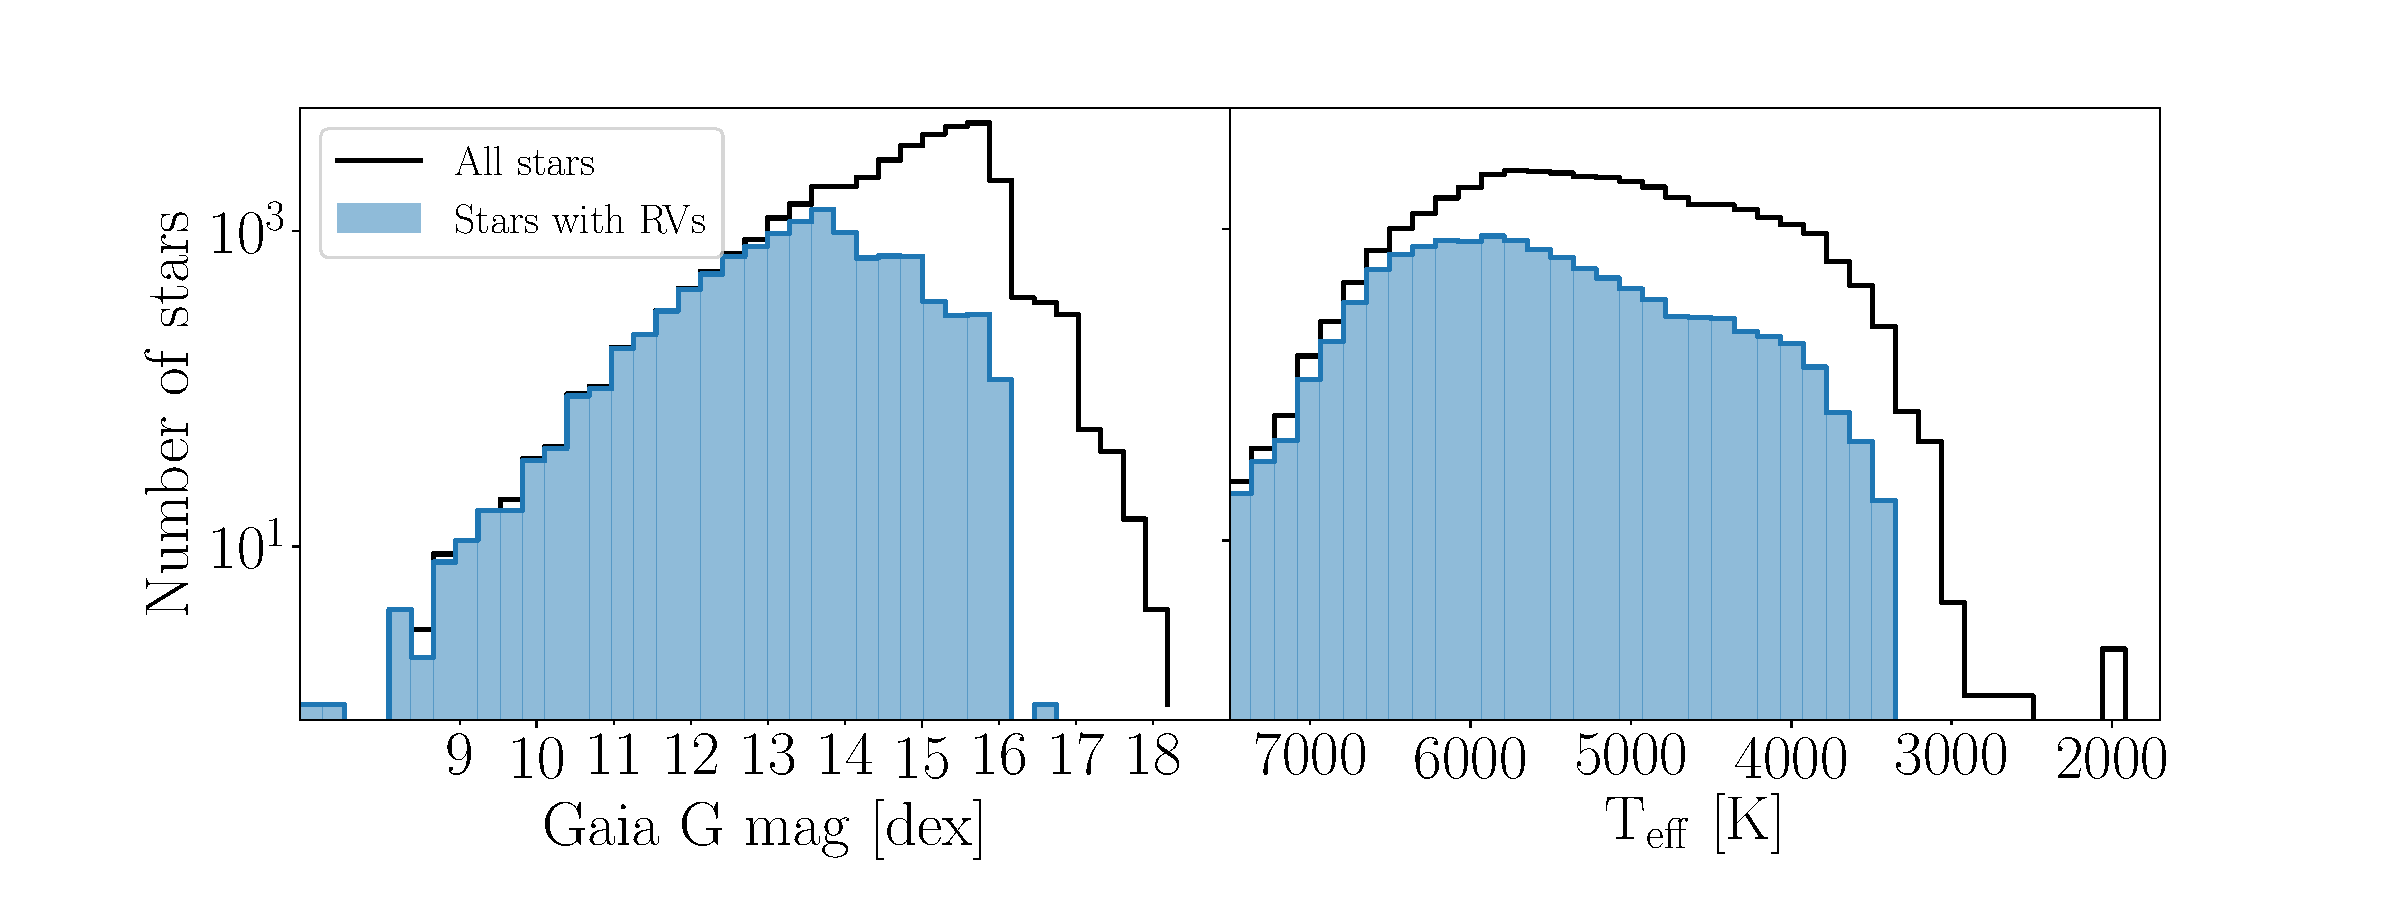
\includegraphics[width=1\textwidth]{rv_histogram}
% \label{fig:rv_histogram}
% \end{figure}
% Given that rotational evolution is particularly poorly understood for M
% dwarfs, the cool stars with missing RVs are arguably the most interesting.
% To fill-in the low-temperature regime, we inferred velocities for stars
% without RV measurements, by marginalizing over missing RVs.
% % \begin{figure}[ht!]
% % \caption{
% % Vertical velocity dispersion as a function of rotation period and effective
% %     temperature for \kepler\ stars with measured rotation periods.
% % Colored points show stars with RV measurements from \gaia\ or \lamost, with
% %     their color indicating their velocity dispersion.
% % Faint grey points show the combined \mct\ and \citet{santos2019} samples,
% %     including stars without RV measurements.
% % The coolest stars in this sample do not have RVs because they are faint.
% % }
% %   \centering 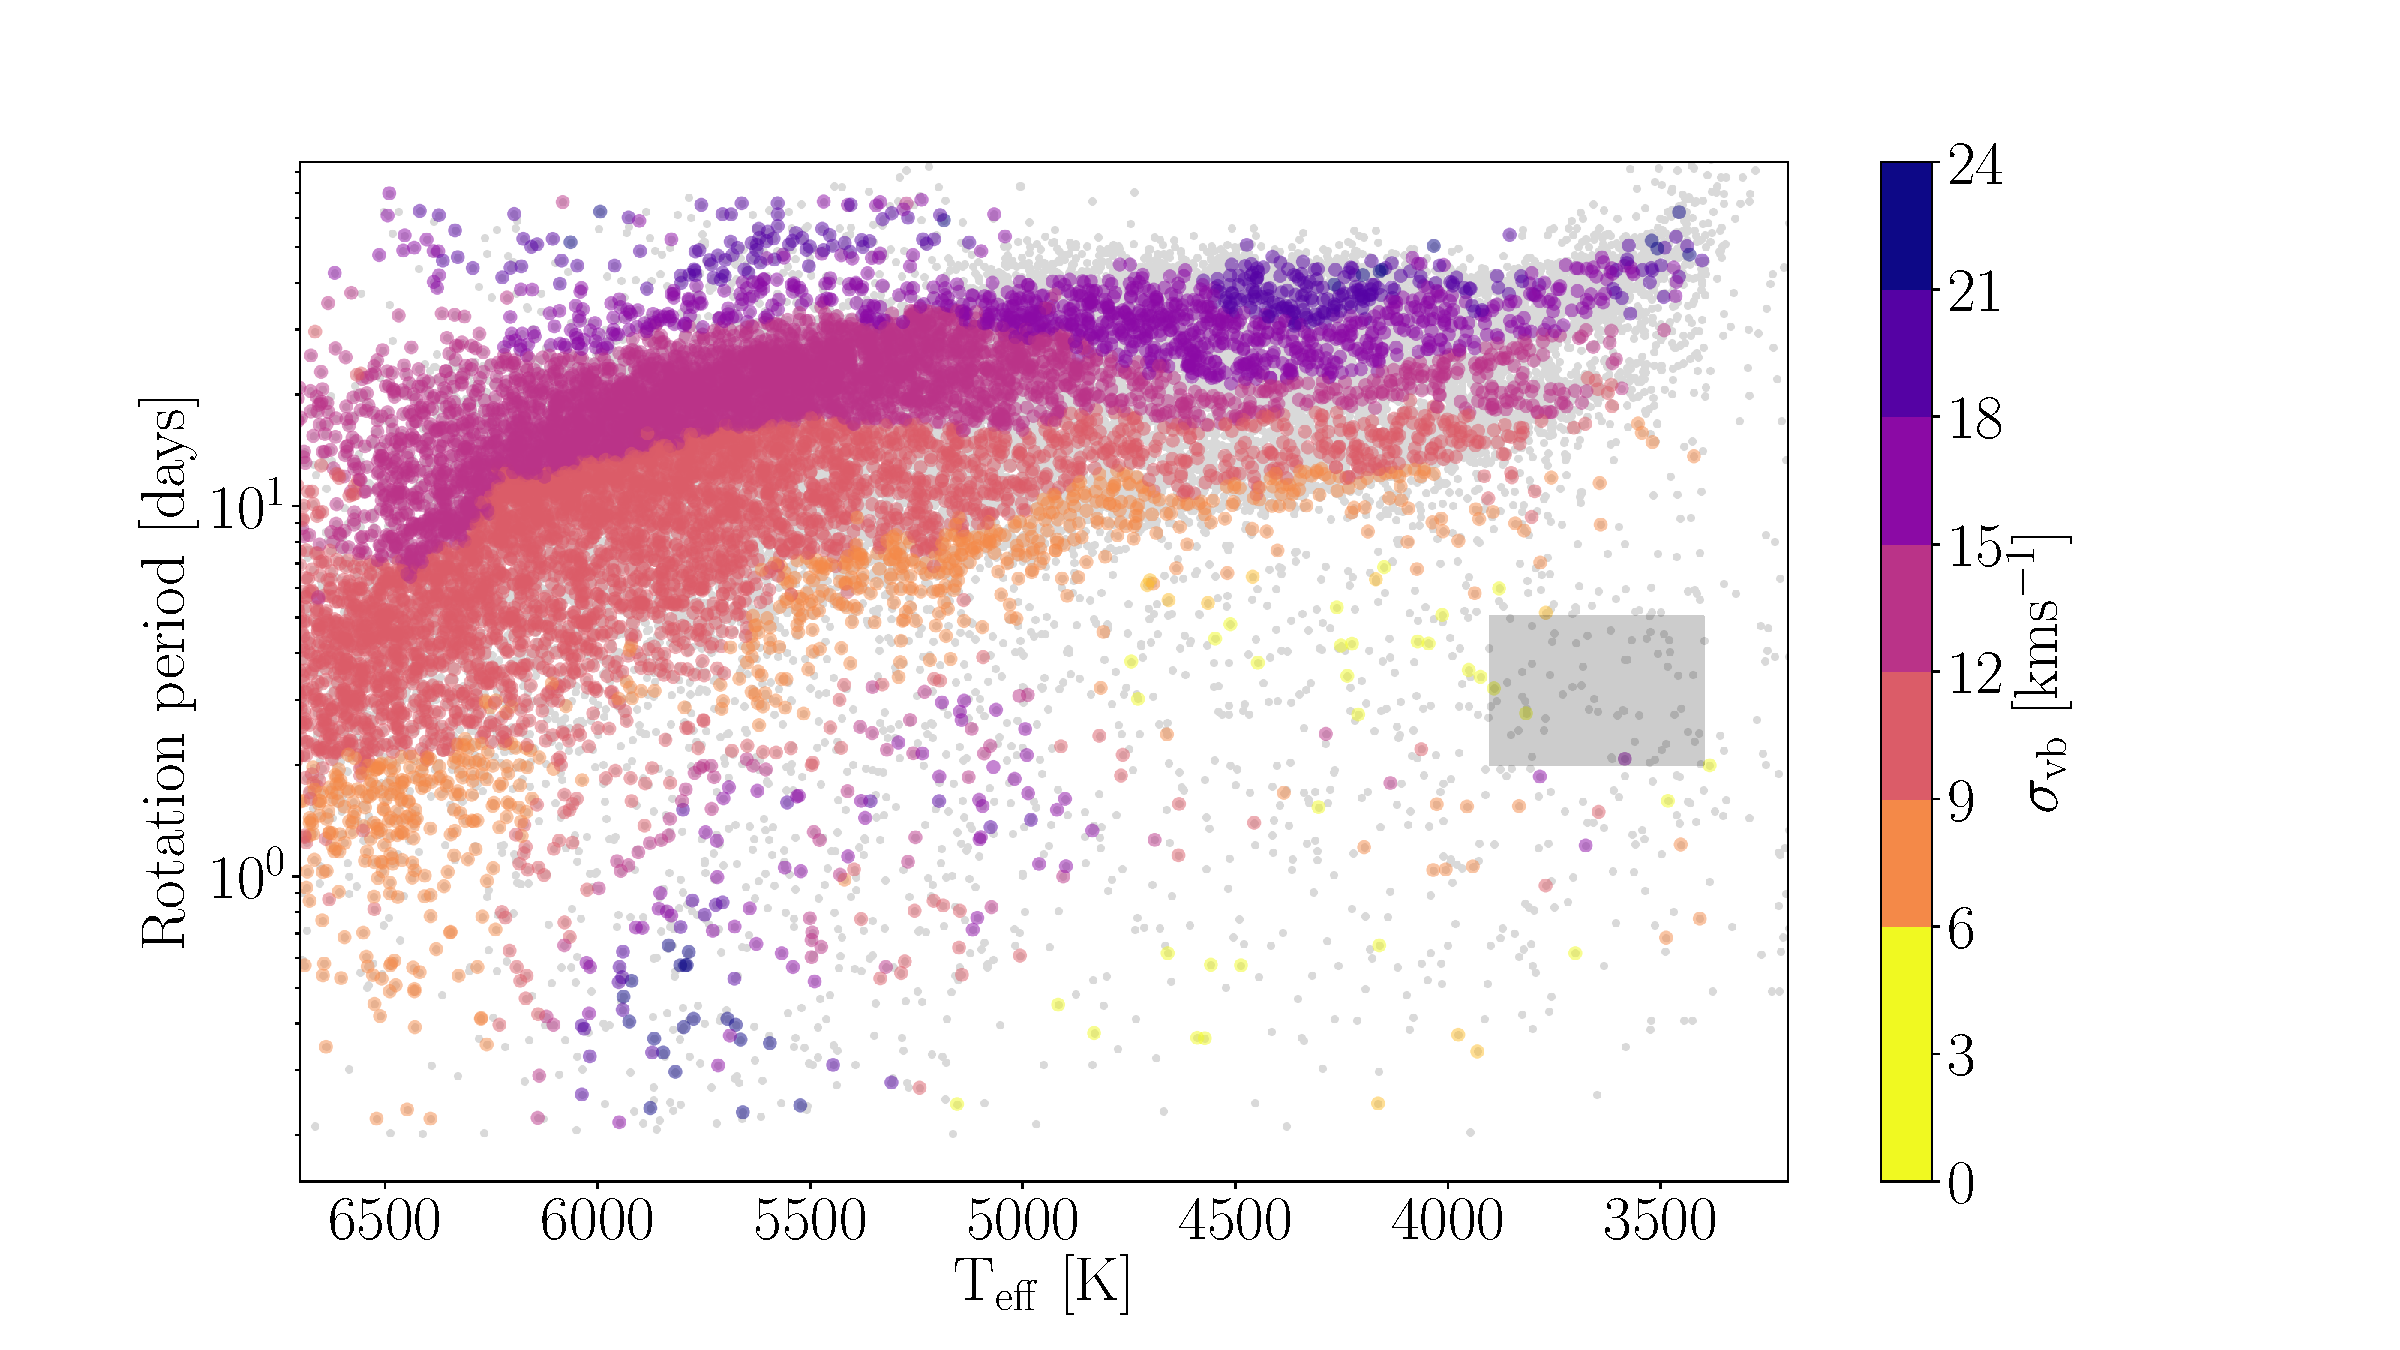
\includegraphics[width=1\textwidth]{existing_rvs}
% % \label{fig:existing_rvs}
% % \end{figure}

\subsection{Inferring 3D velocities (marginalizing over missing RV
measurements)}
\label{sec:inference}

% Three-dimensional velocities in galactocentric coordinates: \vx, \vy, and \vz\
% can only be directly computed via a transformation from 3D velocities in
% another coordinate system, like the equatorial coordinates provided by \gaia:
% \mura, \mudec, and RV.
% For stars with no measured RV in \gaia\ DR2, \vx, vy, and \vz\ can still be
% inferred from positions and proper motions alone, by marginalizing over
% missing RV measurements.
For each star in our sample without an RV measurement, we inferred \vx, \vy,
and \vz\ from the 3D positions (right ascension, \ra, declination, \dec, and
parallax, \parallax) and 2D proper motions (\mura and \mudec) provided in the
\gaia\ DR2 catalog \citep{brown2011}.
We also simultaneously inferred distance, (instead of using inverse-parallax),
to model velocities \citep[see \eg][]{bailer-jones2015, bailer-jones2018}.

Using Bayes rule, the posterior probability of the velocity parameters given
the Gaia data can be written:
\begin{equation}
    p({\bf v_{xyz}}, D | \mu_{\alpha}, \mu_{\delta}, \alpha, \delta, \pi) =
    p(\mu_{\alpha}, \mu_{\delta}, \alpha, \delta, \pi | {\bf v_{xyz}}, D)
    p({\bf v_{xyz}}) p(D),
\end{equation}
where $D$ is distance and ${\bf v_{xyz}}$ is the 3D vector of velocities.
To evaluate the likelihood function, our model predicted observable data from
model parameters, \ie\ it converted \vx, \vy\, \vz\ and $D$ to \pmra, \pmdec\
and \parallax.
In the first step of the model evaluation, cartesian coordinates, \x, \y, and
\z\, were calculated from \ra\ and \dec\ measurements and $D$ ($1/\pi$) for
each star, by applying a series of matrix rotations, and a translation to
account for the Solar position.  The cartesian Galactocentric velocity
parameters, \vx, \vy, and \vz, were then converted to equatorial coordinates,
\pmra\ and \pmdec, via another rotation.

As mentioned previously, the specific positioning of the \kepler\ field (at
low Galactic latitude) allows \vz\ to be well-constrained from proper motion
measurements alone.
This also happens to be the case for \vx, because the direction of the
\kepler\ field is almost aligned with the \y-axis of the Galactocentric
coordinate system and is almost perpendicular to both the \x\ and \z-axes (see
figure \ref{fig:kepler_field}).
For this reason, the \y-direction is similar to the radial direction for
observers near the Sun, so \vy\ will be poorly constrained for \kepler\ stars
without RV measurements.
On the other hand, \vx\ and \vz\ are almost perpendicular to the radial
direction and can be precisely inferred with proper motions alone.
\begin{figure}[ht!]
\caption{
\x, \y\ and \z\ positions of stars observed by \kepler, showing the
    orientation of the \kepler\ field.
The direction of the field is almost aligned with the \y-axis and almost
    perpendicular to the \x\ and \z-axes, which is why \vx\ and \vz\ can be
    tightly constrained for \kepler\ stars without RVs, but \vy\ cannot.
}
  \centering
    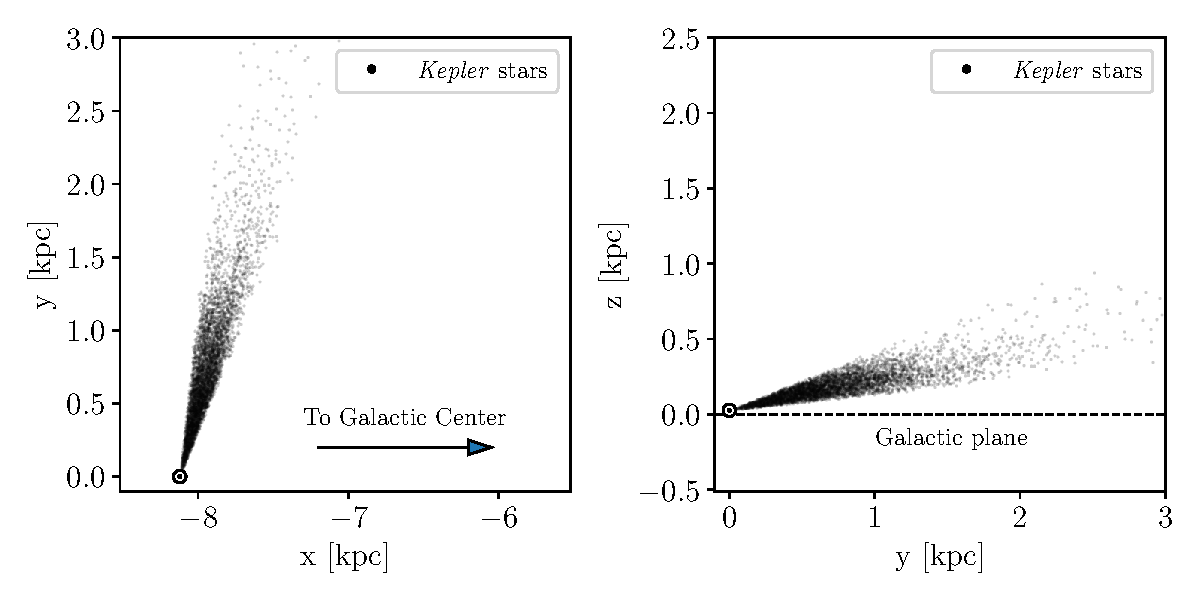
\includegraphics[width=.7\textwidth]{kepler_field}
\label{fig:kepler_field}
\end{figure}

\subsection{The prior}
\label{sec:prior}

The prior distribution over distance and velocities was constructed from the
data.
We calculated the means and covariances of the \vx, \vy, \vz\ and $\ln(D)$
distributions of stars {\it with measured RVs} and then used these means and
covariances to construct a multivariate Gaussian prior over the parameters for
stars {\it without} RVs.
Velocity outliers greater than 3-$\sigma$ were removed before calculating the
means and covariances of the distributions.
The 2-dimensional ln-distance and velocity distributions are displayed in
figure \ref{fig:prior_distributions_2D}, with 2-$\sigma$ contours shown in
blue.
\begin{figure}[ht!]
\caption{
The 2D velocity and distance distributions for stars with RV measurements,
    used to construct a multivariate Gaussian prior over velocity and
    distance parameters for stars {\it without} RVs.
2-$\sigma$ contours are shown in blue.
}
  \centering
    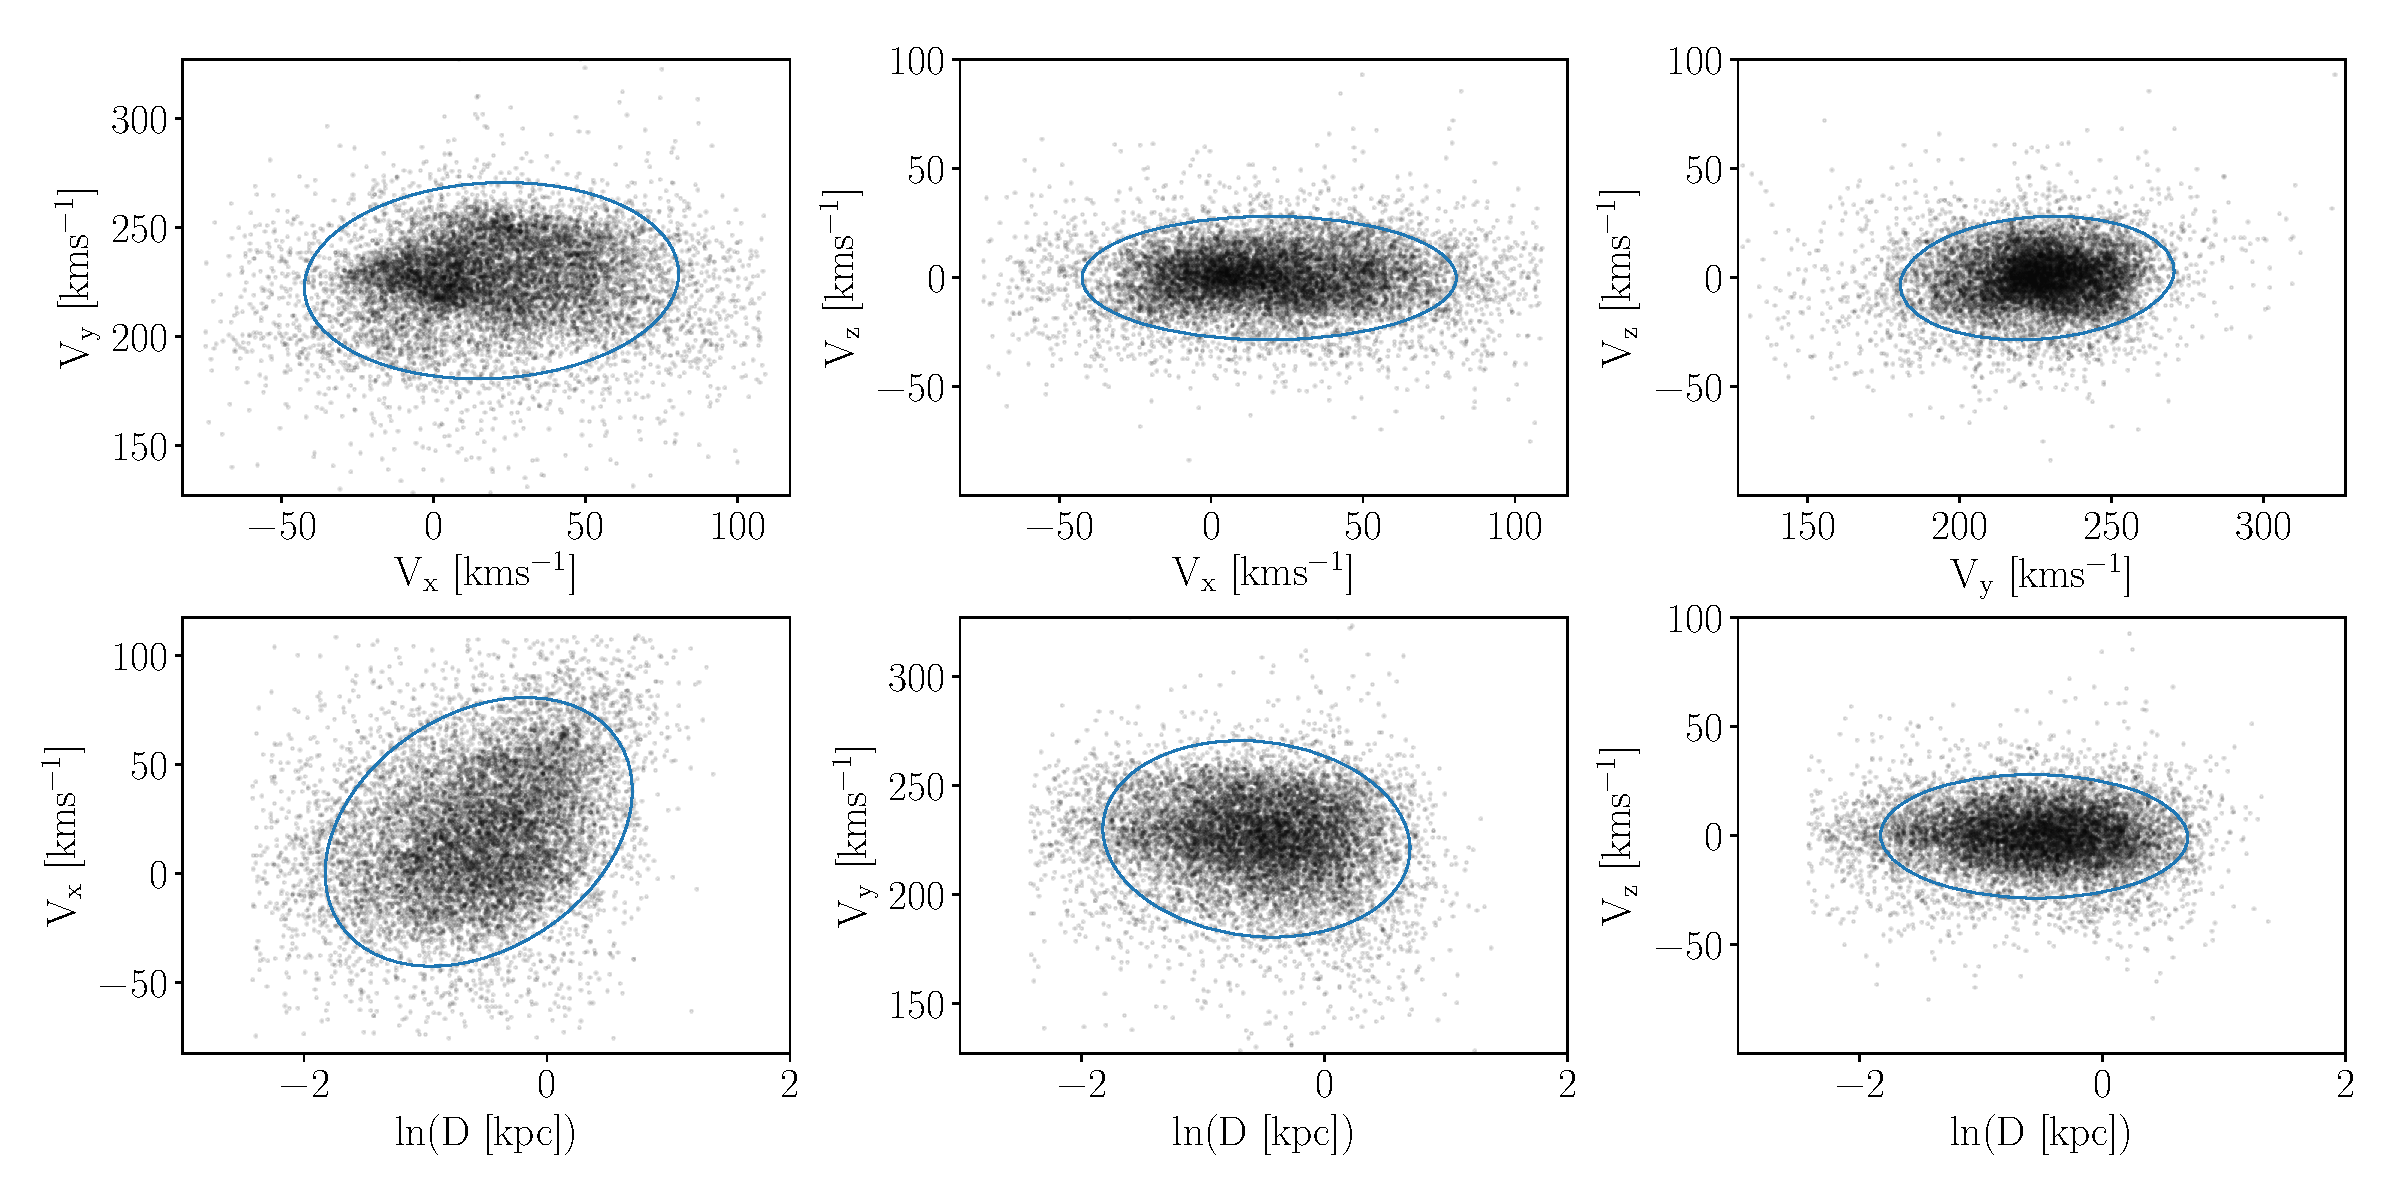
\includegraphics[width=1\textwidth]{prior_distributions_2D}
\label{fig:prior_distributions_2D}
\end{figure}

Our goal was to infer the velocities of stars {\it without} RV measurements
using a prior calculated from stars {\it with} RV measurements.
However, stars with and without RVs are likely to be different populations,
with parameters that depend on the \gaia\ and \lamost\ selection functions.
In particular, stars without RV measurements are more likely to be fainter,
cooler, and further away.
% Lower-mass stars are, on average, older, and have larger velocity dispersions,
% plus stars in different locations in the Galaxy have different orbital
% velocities.
For this reason, a prior based on the velocity distributions of stars with RVs
will not necessarily reflect the velocities of those without.
However, given that \vx\ and \vz\ are strongly informed by proper motion
measurements, and therefore likely to be relatively prior-insensitive, the
prior may not impact our final vertical velocity, and subsequent kinematic
ages, significantly.
Remember, we are mainly interested in the \vz\ parameter because {\it
vertical} velocity dispersion is a well-studied age indicator.

We tested the influence of the prior on the velocities we inferred.
One of the main features of the \gaia\ and \lamost\ RV selection functions is
brightness: \gaia\ DR2 RVs are only available for stars brighter than around
13th magnitude, and \lamost\ RVs for stars brighter than around 17th
magnitude.
\racomment{Ruth, check the actual LAMOST selection function.}
For this reason, we tested priors based on stellar populations with different
apparent magnitudes.
Three priors were tested: one calculated from the velocity distributions of
the brightest half of the RV sample (\gaia\ $G$-band apparent magnitude $<$
13.9), one from the faintest half ($G$ $>$ 13.9), and one from all stars with
RVs.
Figure \ref{fig:prior_distributions} shows the distributions of the faint
(blue) and bright (orange) halves of the RV sample as kernel density estimates
(KDEs).
The distributions are different because bright stars are more massive,
younger, and closer to the Sun on average than faint stars.
As a result, these stars occupy slightly different Galactic orbits.
The Gaussian fits to these distributions, which were used as prior PDFs, are
shown in figure \ref{prior_distributions} as dashed, colored lines.
The Gaussian fit to {\it all} the data, both bright and faint, is shown as a
black solid line.
The means of the faint and bright distributions differed by 6 \kms, 5 \kms, 1
\kms\ and 0.21 kpc, for \vx\, \vy, \vz\ and $\ln(D)$, respectively.
The \vx, \vy, and distance distributions of these stars are strongly dependent
on brightness.
However, the \vz\ distribution does not vary significantly with stellar
brightness.
Since \vz\ is the only velocity we actually used to infer kinematic ages, this
indicates that the choice of prior does not strongly impact our final results.
To confirm this, we tested the influence of the prior on the parameters.
% The black Gaussian, fit to the entire RV sample, is the prior we ended up
% using in our model.

\begin{figure}[ht!]
\caption{
    Velocity and distance distributions of faint (blue) and bright (orange)
    stars with RVs, shown as KDEs.
    Gaussian fits to these distributions are shown as dashed lines in
    corresponding colors.
    The solid black line shows the Gaussian fit to all data (bright and faint
    combined) and is the prior we ended up using in our model.
}
  \centering
    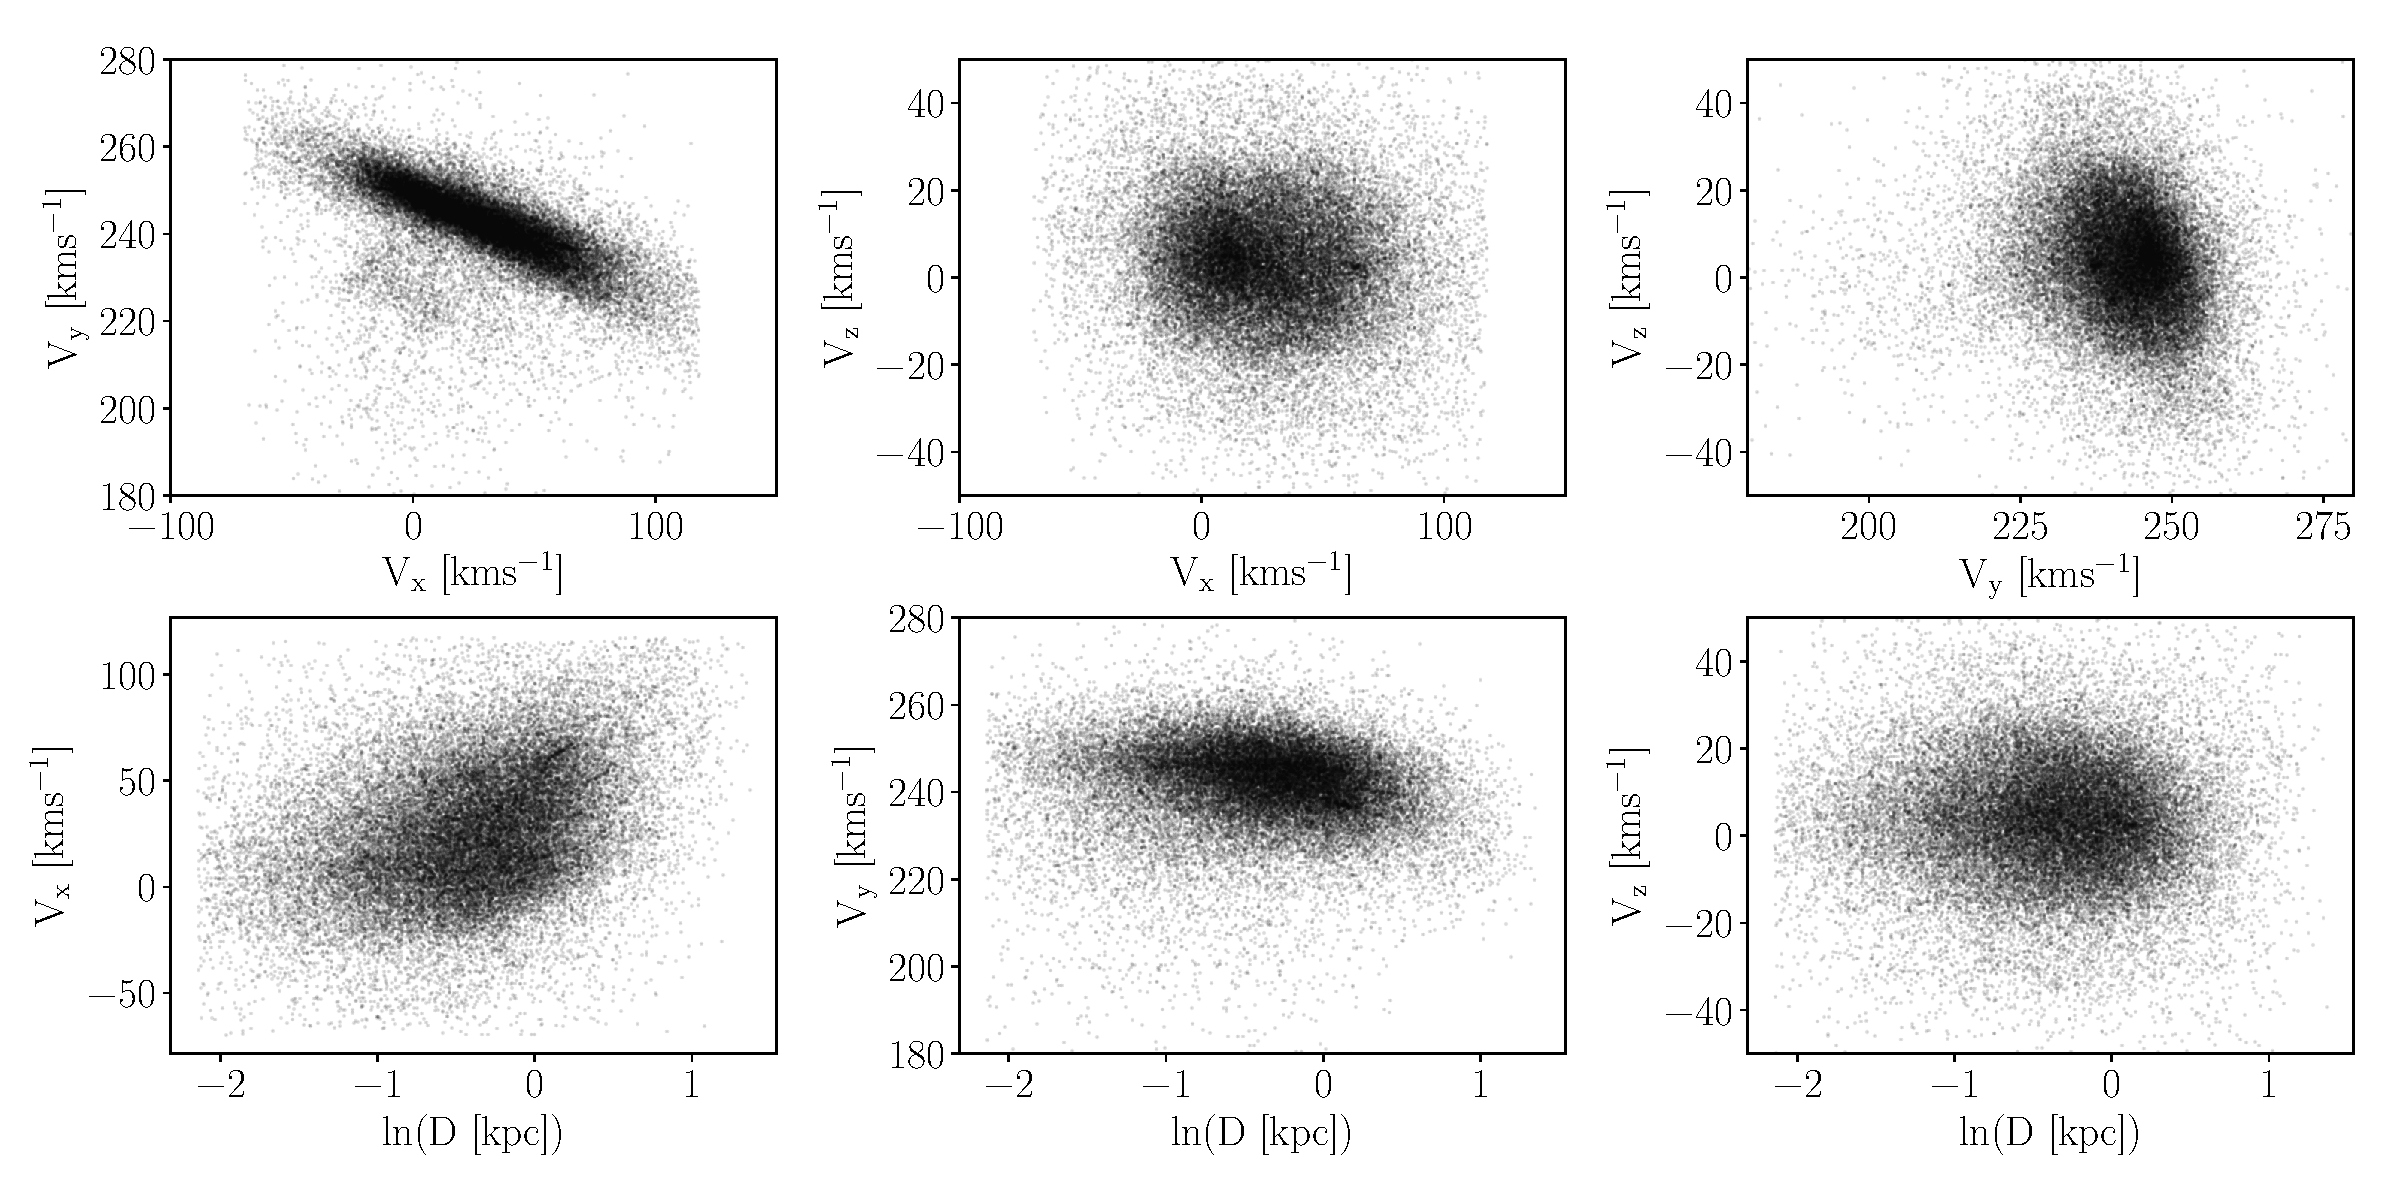
\includegraphics[width=1\textwidth]{prior_distributions}
\label{fig:prior_distributions}
\end{figure}
We inferred the velocities of 3000 stars chosen at random from the
\gaia-\lamost\ RV sample using each of these three priors and compared the
inferred velocity distributions.
If the inferred velocities were highly prior-dependent, the resulting
distributions, obtained from different priors, would look very different.
The results of this test are shown in figure \ref{fig:prior_comparison}.
From left to right, the three panels show the distributions of inferred \vx,
\vy, and \vz.
The blue dashed line shows a KDE, representing the
distributions of velocities inferred using the prior calculated from the faint
half of the RV sample.
Similarly, the solid orange line shows the distribution of inferred velocities
using the prior calculated from the bright half of the RV sample, and the
solid black line shows the results of the prior calculated from {\it all}
stars with measured RVs.

The median values of the \vy\ distributions, resulting from the faint and
bright priors, differ by around 4 \kms.
This is similar to the difference in means of the faint and bright populations
(5 \kms, as quoted above).
The inferred \vx\ and \vz\ distributions differ by 2 \kms\ and 0.3 \kms,
respectively.
Regardless of the prior choice, the \vx\ and \vz\ distributions are similar
because velocities in the \x\ and \z-directions are not strongly prior
dependent: they are tightly constrained with proper motion measurements alone.
However, the distribution of inferred \vy\ velocities {\it does} depend on the
prior.
This is because the \y-direction is close to the radial direction for \kepler\
stars (see figure \ref{fig:kepler_field}), and \vy\ cannot be tightly
constrained without an RV measurement.
% It is therefore highly dependent on the prior.
\begin{figure}[ht!]
\caption{
The distributions of velocity and distance parameters, inferred using three
    different priors.
The orange line is a KDE that represents the distribution of parameters
    inferred with a Gaussian prior, estimated from the bright half of the RV
    sample ($G < $ 13.9).
The blue dashed line shows the results from a prior estimated from the faint
    half of the RV sample ($G > 13.9$.
The black line shows the results from a prior calculated from all stars with
    RV measurements and is the prior we adopt in our final analysis.
    }
  \centering
    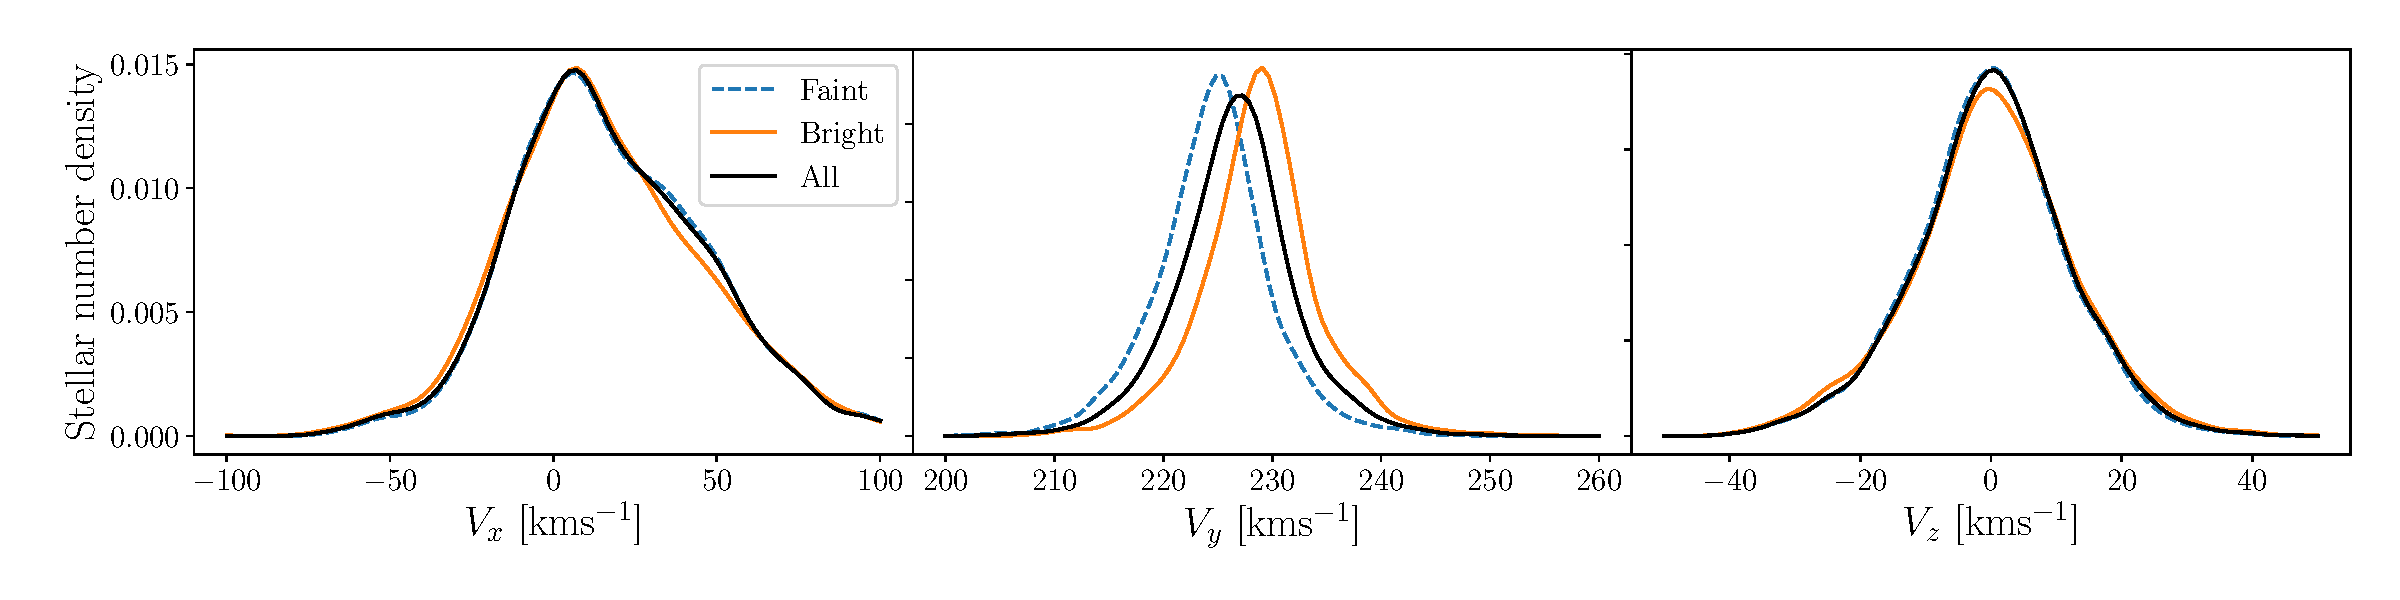
\includegraphics[width=1\textwidth]{prior_comparison}
\label{fig:prior_comparison}
\end{figure}

% Fainter stars have smaller y-velocities than brighter stars because they are,
% on average, further from the Sun

Although this test was performed on stars with RV measurements, which are
brighter overall than the sample of stars without RVs (\eg\ figure
\ref{fig:rv_histogram}), figure \ref{fig:prior_comparison} nevertheless shows
that \vx\ and \vz\ are not strongly prior-dependent.
In this work we are only concerned with \vz, as we only use {\it vertical}
velocity dispersion as an age indicator.
The difference in the dispersions of \vz\ velocities, calculated with the
three different priors tested above was smaller than 0.5 \kms.
We therefore conclude that vertical velocity dispersion is relatively
insensitive to prior choice, and we adopt a prior calculated from the
distributions of all stars with RV measurements (black Gaussians in figure
\ref{fig:prior_comparison}).

% \begin{figure}[ht!]
% \caption{
%     }
%   \centering
%     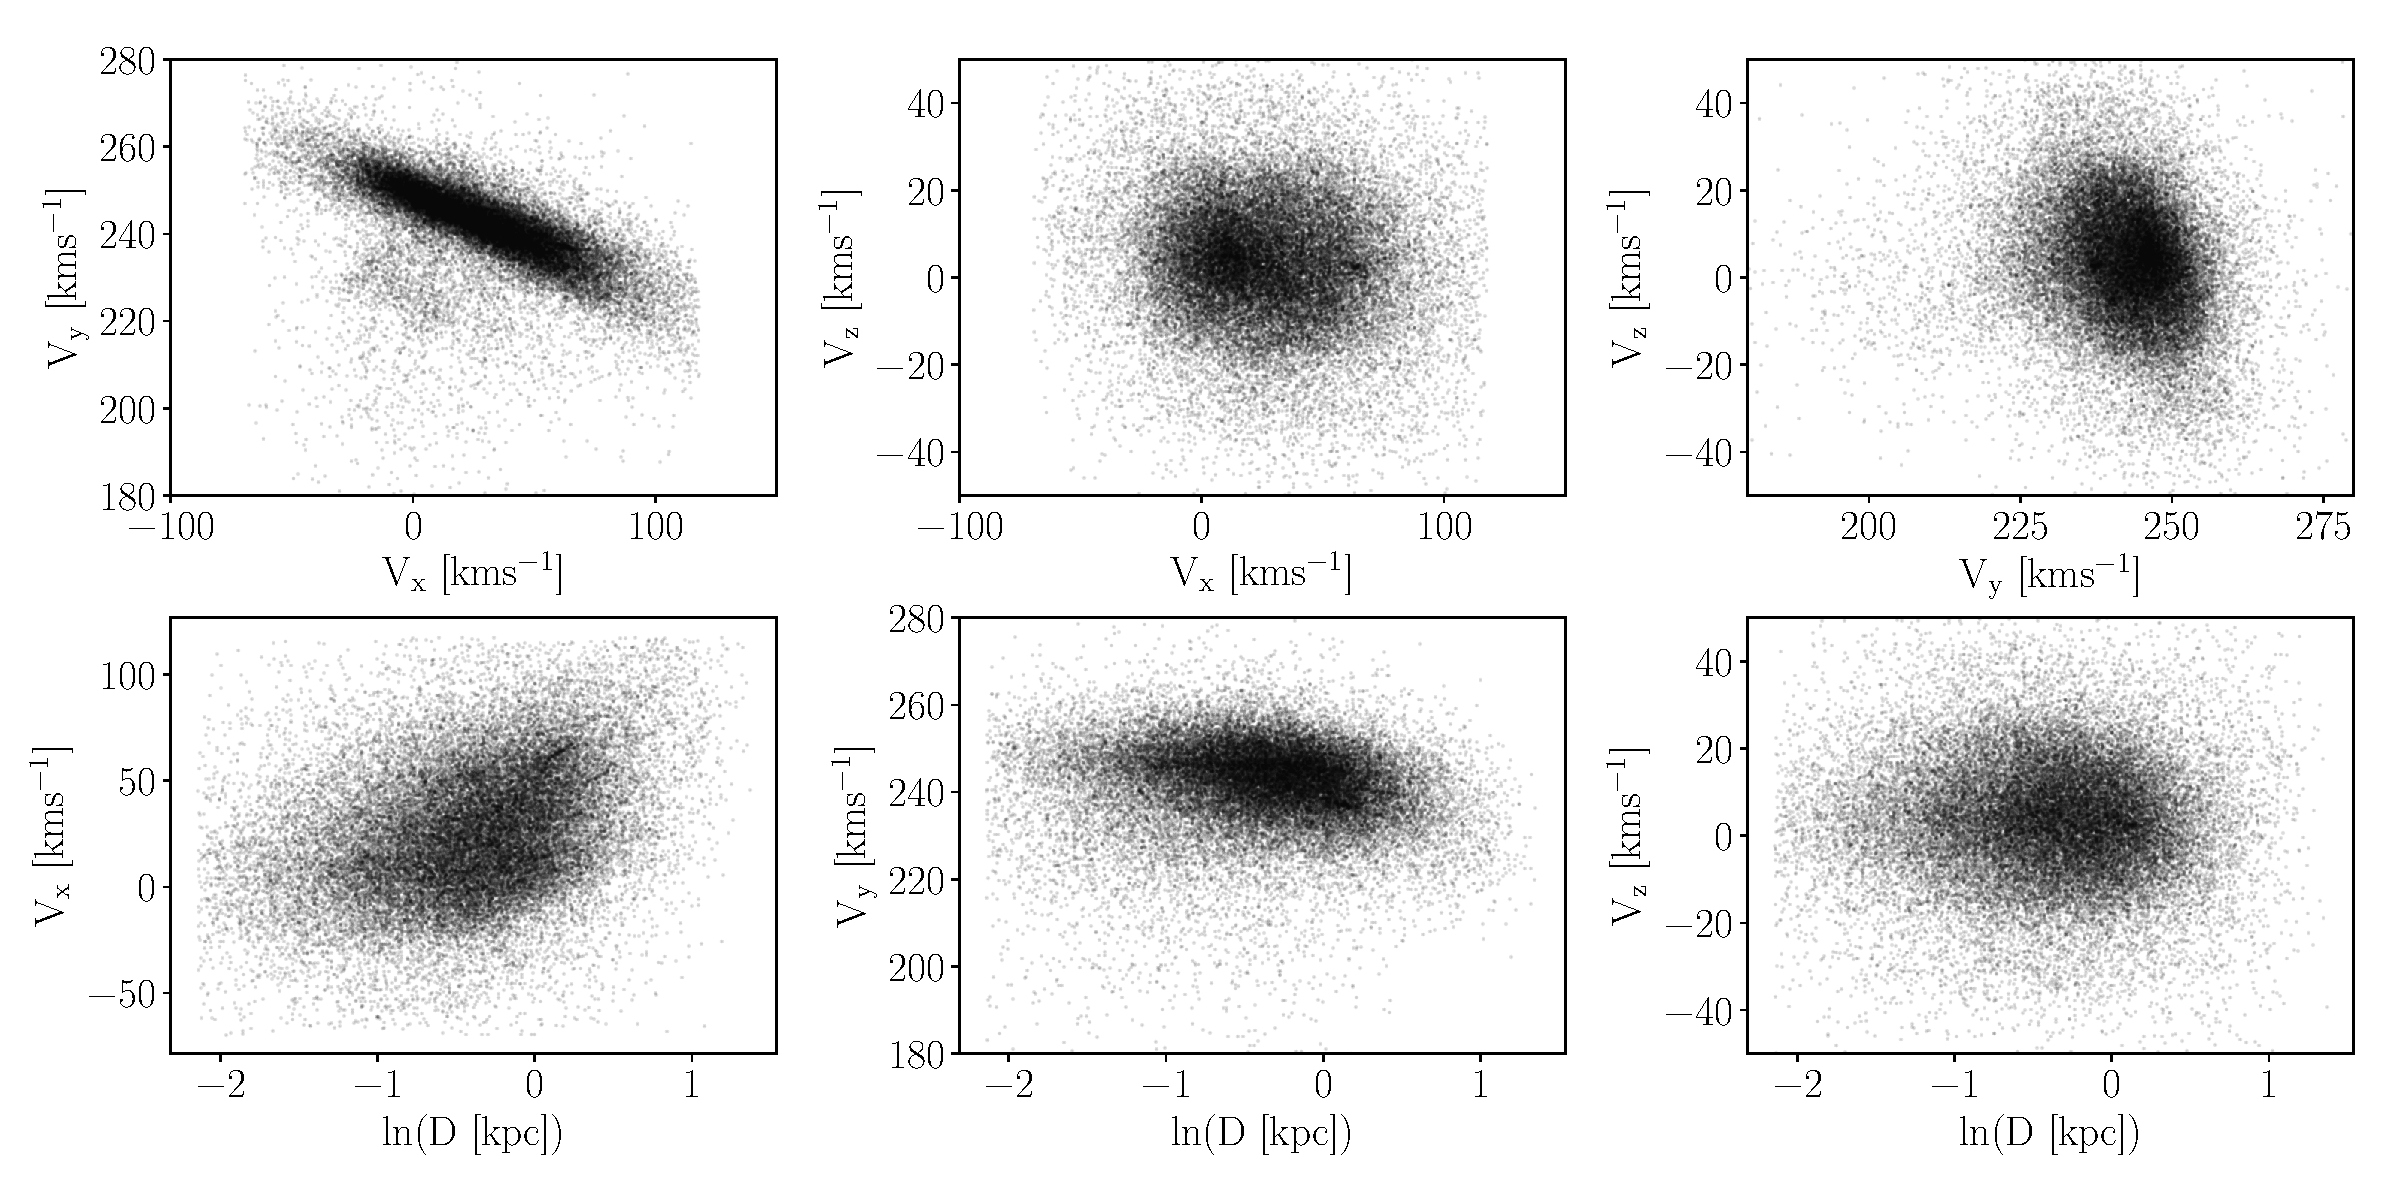
\includegraphics[width=1\textwidth]{prior_distributions}
% \label{fig:prior_distributions}
% \end{figure}

\subsection{Inferred velocities}

For each star in the \kepler\ field, we explored the posteriors of the four
parameters, \vx, \vy, \vz, and $\ln(D)$ using the {\it PyMC3} No U-Turn
Sampler (NUTS) algorithm, and the {\tt exoplanet} \python\ library
\racomment{(citations)}.
We tuned the {\it PyMC3} sampler for 1500 steps, with a target acceptance
fraction of 0.9, then ran four chains of 1000 steps for a total of 4000 steps.
Using PyMC3 made the inference procedure exceptionally fast -- taking just a
few seconds per star on a laptop.
\racomment{Check what convergence criteria you should use, or justify these
choices.}

To validate our method, we inferred velocities for stars in our sample with
measured RVs and compared those inferred values with velocities calculated
directly from 6D position, proper motion, and RV measurements.
Figure \ref{fig:residuals} shows the \vx, \vy\ and \vz\ velocities we
inferred, for 3000 stars chosen at random, compared with those calculated from
measured RVs.
\begin{figure}[ht!]
\caption{Vertical velocities calculated with full 6D information vs vertical
    velocities inferred without RVs, for 3000 \mct\ stars with \gaia\ RV
    measurements.}
  \centering
    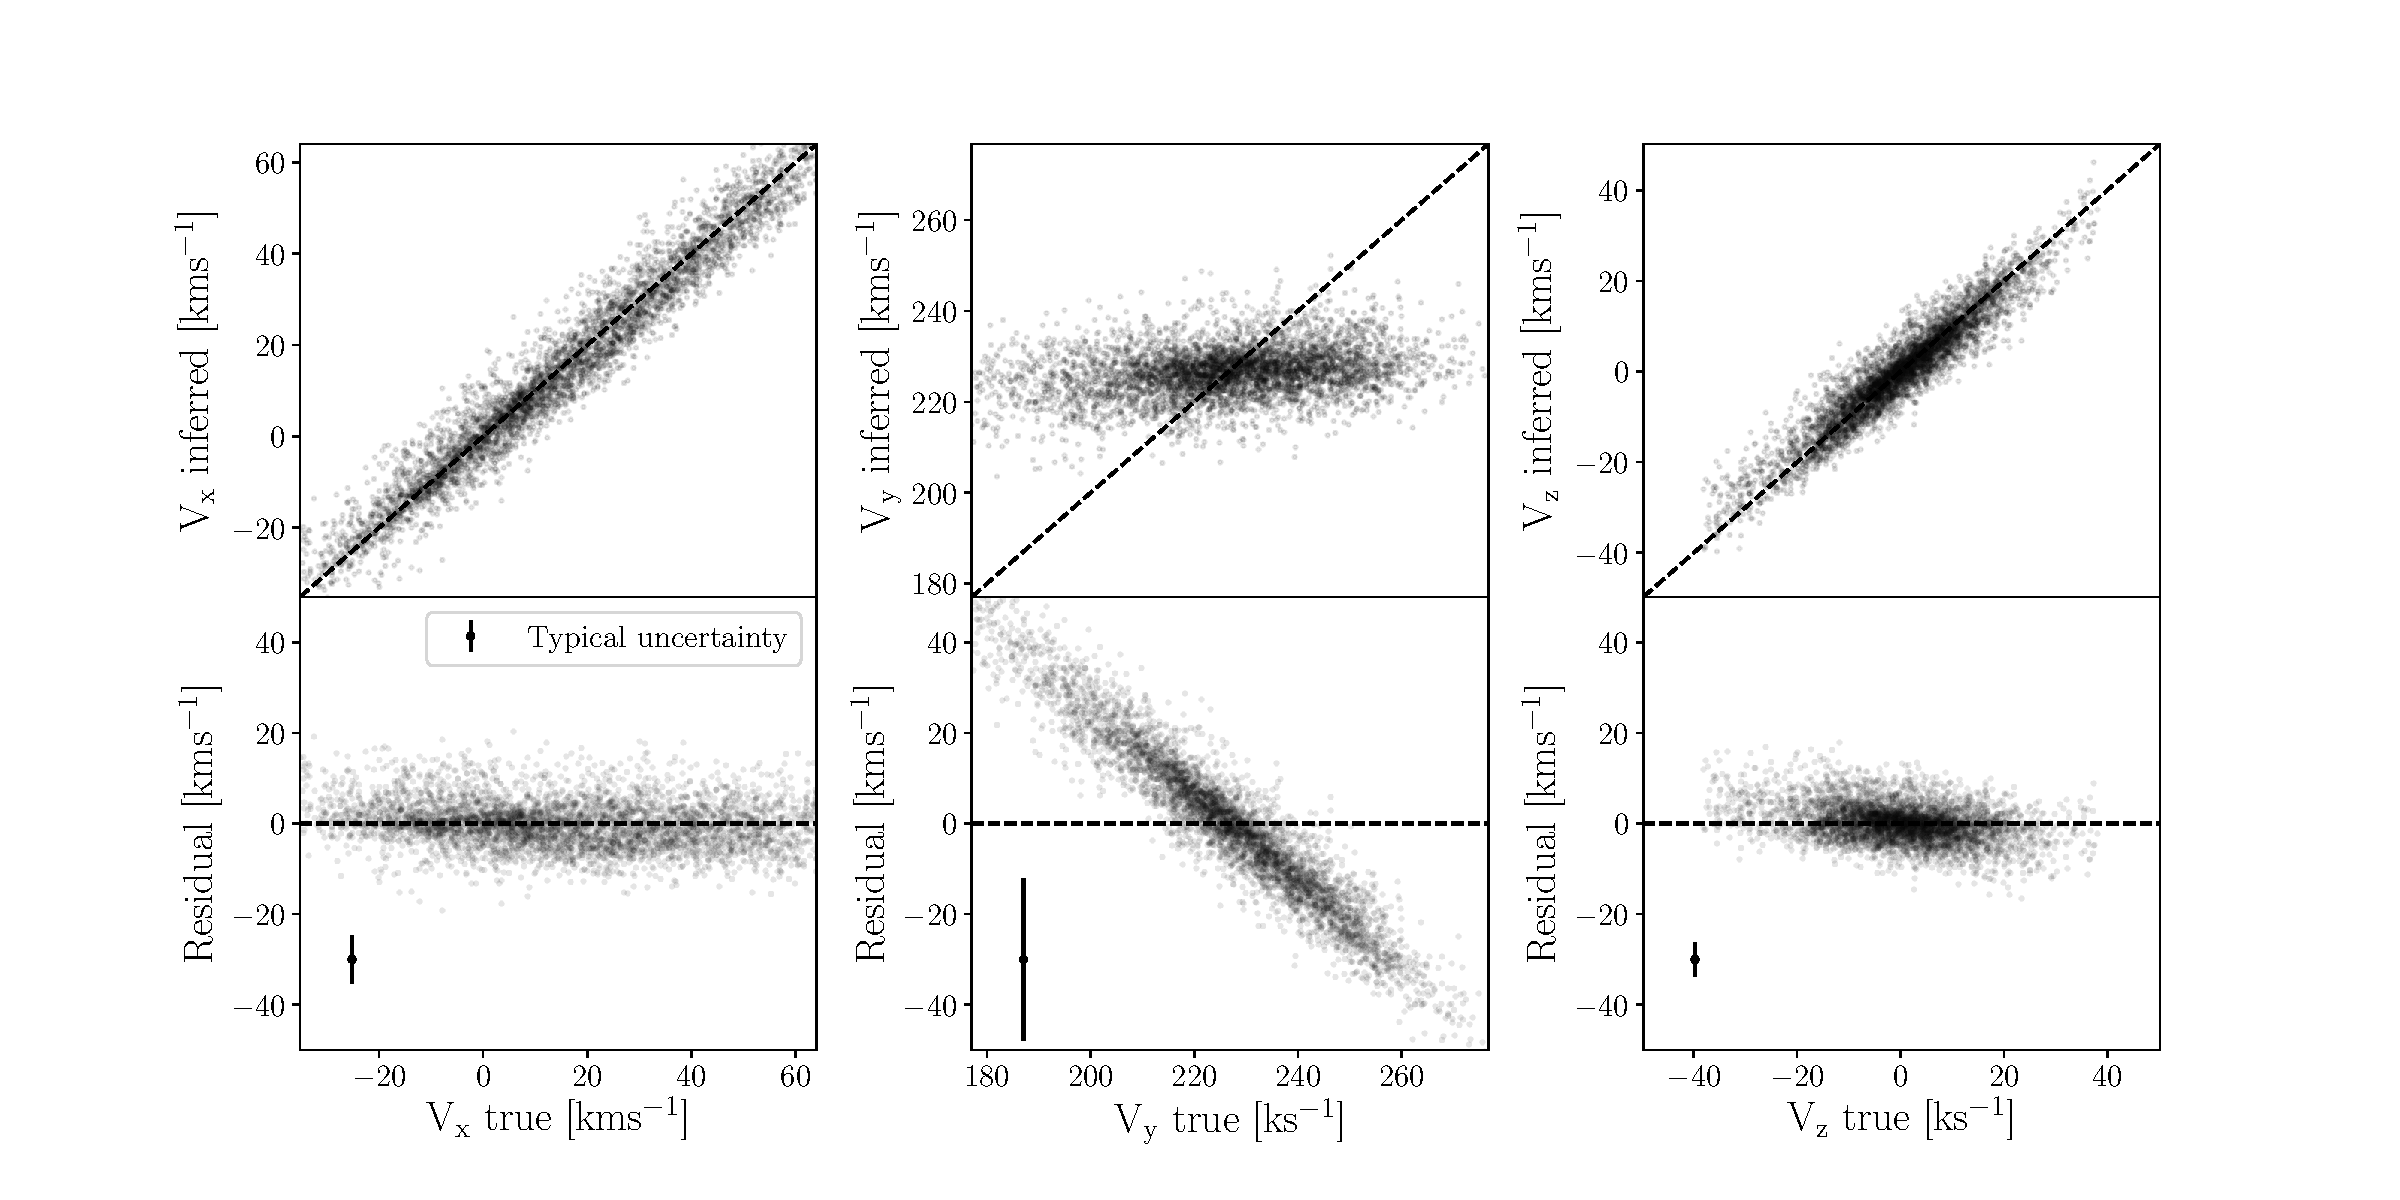
\includegraphics[width=1\textwidth]{residuals}
\label{fig:residuals}
\end{figure}

The three velocity components, \vx, \vy\ and \vz\ were recovered with
differing levels of precision: \vx\ and \vz\ are inferred more precisely than
\vy.
This is because of the orientation of the \kepler\ field, shown in figure
\ref{fig:kepler_field}.
\racomment{Slight inaccuracies seen in the residual panels for \vx\ and \vz\
are caused by ....
Quote some summary statistics.}



\section{Kinematic ages}
\subsection{Calculating velocity dispersions}
\label{sec:velocity_dispersion}

A kinematic age can be calculated from the velocity dispersion, \ie\ standard
deviation, of a group of stars.
These velocity dispersions can then be converted into an age using an AVR
\citep[\eg][]{holmberg2009, yu2018}.
Kinematic ages represent the {\it average age} of a group of stars and are
most informative when stars are grouped by age.
If a group of stars have similar ages, their kinematic age will be close
the age of each individual.
On the other hand, the kinematic age of a group with large age variance will
not provide much information about the ages of individual stars.
Velocity distributions themselves do not reveal whether a group of stars have
similar or different ages, since either case the velocities are
Gaussian-distributed.
Fortunately however, we can group \kepler\ stars by age using the implicit
assumption that underpins gyrochronology: that stars with the same rotation
period and color are the same age.
We discuss the implications of this assumption and cases where it doesn't
apply in the Discussion of this paper (section \ref{sec:discussion}).

In this paper, we calculated the kinematic age of {\it each individual star}
in our sample, by grouping it with its neighbors in \logp--\teff\ space.
This method is similar to calculating a rolling, or running standard
deviation and allowed us to assign a unique age to each star.
However, ages calculated this way are tightly correlated, and their
correlation depends strongly on window-size.

% To calculate a \vz\ velocity dispersion and kinematic age for each \kepler\
% rotator, we grouped stars with their neighbors in \logp--\teff\ space.
We tested two methods of grouping stars: K-nearest neighbors, and bins in
\logp\ and \teff .
In the K-nearest neighbors method, each star was grouped with the K-nearest
stars in \logp-\teff\ space.
Groups created this way spanned a small \logp -\teff\ range where the stellar
number density was large, and a large range where the number density was
small.
In other words, the number of stars was fixed but the window-size changed.
In the fixed range method, stars were grouped within a fixed \logp -\teff
window.
This method created groups with large numbers of stars in densely populated
regions of the \logp--\teff\ plane, and small numbers of stars in sparsely
populated regions, \ie\ the number of stars changed but the window-size was
fixed.
To choose the best method, and to optimize for the parameters of each (K and
window-size), we conducted a set of tests.

\subsection{Converting velocity dispersion to age with an AVR}
\label{sec:avr}
We used the \citet{yu2018} AVR to convert velocity dispersion to age.
This relation was calibrated using the ages and velocities of red clump stars.
They divided their sample into metal rich and poor subsets, and calibrated
separate AVRs for each, plus a global AVR.
Their AVR is a power law:
\begin{equation}
    \sigma_{vz} = \alpha t ^\beta,
\end{equation}
where $\alpha$ and $\beta$ take values (6.38, 0.578) for metal rich stars
(3.89, 1.01) for metal poor stars, and (5.47, 0.765) for all stars.

We used 1.5$\times$ the Median Absolute Deviation (MAD) of velocities, which
is a robust approximation to the standard deviation and is less sensitive to
outliers.
Velocity outliers could be binary stars or could be generated by
underestimated parallax or proper motion uncertainties.

\subsection{Comparing kinematic ages with asteroseismic and cluster ages}

\subsection{A Gaussian process gyrochronology relation}
\label{sec:gp_model}


\subsection{Calibrating a new gyrochronology relation}
\label{sec:calibration}

To calibrate a new gyrochronology relation we fit an empirical power-law
relation, augmented with a Gaussian process, to a grid of kinematic ages and
open cluster stars.
These cluster stars have precise rotation periods measured from Kepler and K2
light curves, and well-determined ages from cluster-based isochrone fitting.
In this section we describe how we fit our model to these data.

\subsubsection{The model}

To calibrate a new empirical gyrochronology relation
we used a composite model, consisting of an underlying mean function,
augmented with a Gaussian process.
The mean function is similar to previous empirical gyrochronology models and
consists of two separable power-law relations: one describing the relationship
between rotation period and age, and the other between rotation period and
color \citep[\eg][]{barnes2003, barnes2007, mamajek2008, meibom2015, angus2015,
angus2019}.

Our mean function is comprised of a single power-law in age, $f(t)$, and a
broken power law in color, $g(C)$:
\begin{equation}
P_\mathrm{rot} = f(t) + g(C),
\end{equation}
where $P_\mathrm{rot}$ is rotation period in days, $t$ is age in Gyr, and C is
Gaia color: $\mathrm{G_{BP} - G_{RP}}$.
The age power-law is defined as,
\begin{equation}
f(t) = at^n,
\end{equation}
following the functional form first described in \citep{barnes2003}, where $a$
and $n$ are free parameters.
The broken power-law in color is defined as,
\begin{equation}
g(C) = \delta
\left(\frac{m_1}{1 + e^{s \delta}}\right)
+ \left(\frac{m_2}{1 + e^{-s \delta}}\right),
\end{equation}
where $s$ is a parameter that determines how smooth the break is, $m_1$ is the
slope below (bluewards of) the power-law break, $m_2$ is the slope above
(redwards of) the break, and
\begin{equation}
\delta = C - C_\mathrm{break},
\end{equation}
where $C_\mathrm{break}$ is the color of the power-law break.
In this model, $s$, $m_1$, $m_2$, and $C_\mathrm{break}$ were all free
parameters.

A Gaussian process model then distorts this mean model to provide a better fit
to the data.
In other words, it models the residuals between the mean model and the data.
We used a simple squared exponential kernel function which has only two free
parameters, an amplitude, $A$ and a length scale, $l$.
This kernel function is defined as,
\begin{equation}
k_{ij} = A \exp\left[{\frac{-(x_i - x_j)^2}{2l^2}}\right]
\end{equation}

The parameters were optimized using the {\tt exoplanet} code \citep{exoplanet}.
% The posterior PDFs of these parameters of the power-law relations, and the
% hyper-parameters of the GP kernel were explored with MCMC.
% We used the {\tt exoplanet} \citep{exoplanet} and {\tt PyMC3} \citep{pymc3}
% Python packages to fit this model to the data.

\subsubsection{Formatting the data}

A Gaussian process is only an appropriate model for data generated by a
Gaussian process.
Data with large numbers of outliers or with inaccurately estimated
uncertainties are not Gaussian-distributed and therefore cannot be described
with a Gaussian process.
Rotation period measurements are rarely generated by a Gaussian process for
two main reasons.
Firstly, the uncertainties on rotation period measurements can rarely be
described as Gaussian because they are often plagued by harmonics/aliases and
spurious measurements.
Secondly, the relationship between rotation period and color often has a large
amount of intrinsic scatter.
The is especially true for young stars and M dwarfs, where there is little
correlation between rotation period and age.
This scatter is not generated purely by measurement uncertainties which means
that it is not well-described by a Gaussian process.
This non-Gaussian nature of rotational data necessitated a certain amount of
data formatting or `massaging' in order to fit our model to the data.
We acknowledge that some of the choices we make during this stage are somewhat
arbitrary, and other choices may have worked equally well.
However, in the end our goal was to produce a gyrochronology model that is
reasonably representative of the data.

There are three main approaches we took:
\begin{itemize}
\item {\bf Trimming the cluster data}.
We used a number of open clusters to calibrate our model: Praesepe, the
Hyades, NGC 6811, NGC 6819, and Ruprecht 147.
Although the rotation periods of most G and K stars in these clusters fall on
a tight sequence, Praesepe contains a number of M dwarfs with measured periods
that are highly stochastic.
Given that the scatter in M dwarf rotation periods is intrinsic: it is not
produced by measurement uncertainties, these data are not well-described by a
Gaussian process.
For this reason, we removed M dwarfs with stochastic rotation periods from our
calibration sample.
We removed all cluster stars with rotation periods shorter than one day and
\gcolor\ $>$ 2.2.
We also removed cluster stars with {\it both} \prot\ $<$ 11 days {\it and}
\gcolor\ $>$ 1.5.
Although the Pleiades cluster contains a number of stars with measured
rotation periods, it is too young to have enough members that have converged
onto a tight rotation sequence so we were unable to include it in our
calibration sample in this work.
\racomment{Will probably need to include Pleiades at some point!}

\item {\bf Applying cuts to the kinematic data.}
As with the cluster data, the kinematic data also needed to be Gaussian
distributed.
For this reason, we removed stars whose rotation periods are not
determined by their age and color.
This includes subgiants, young stars, and binaries.
Subgiants were cut by removing stars with Gaia $M_G$ absolute magnitude less
than 4 \racomment{check this}, and stars with {\it both} \gcolor\ $<$ 1.5 {\it
and} kinematic age $>$ 6 Gyr.
Binaries were cut by fitting a 6th order polynomial.... etc.
Here we define `young stars' to mean stars that are too young to have
converged onto the slow rotator sequence.
These stars have rotation periods shorter than the bulk of the rotation period
distribution.
These young stars were removed by calculating their gyro-ages according to the
\citet{angus2019} empirical relation, and then excluding stars with gyro-ages
younger than 0.7 Gyr.
Hot stars...

\item {\bf Converting kinematic data to a grid.}
Once applying these cuts, 20,000 kinematic stars remained.
        Given that fitting a GP to such a large dataset is computationally
        expensive, and given that 20,000 stars is far more than necessary to
        obtain a reasonably accurate gyrochronology model, it made sense to
        reduce this data set in one of two ways.
        We could either have simply subsampled the data, however this would
        have thrown away
        information, so we opted instead to take averages of kinematic ages
        over a grid in rotation period and temperature.
This provides the additional advantage of reducing the age uncertainties by
        the square root of the number of data points.
        This was beneficial because we did not include age uncertainties in
        our fit (so the smaller the age-uncertainties the better).
Secondly, we were not including age uncertainties in our fit.
For the clusters we can maybe get away with this, but the uncertainties on the
kinematic are non-negligable \citep[likely 1-2 Gyr][]{lu2021}).
To get around this issue, instead of fitting our GP model to the raw data, we
instead converted it to a grid.
\end{itemize}

\begin{figure}
\caption{
}
  \centering 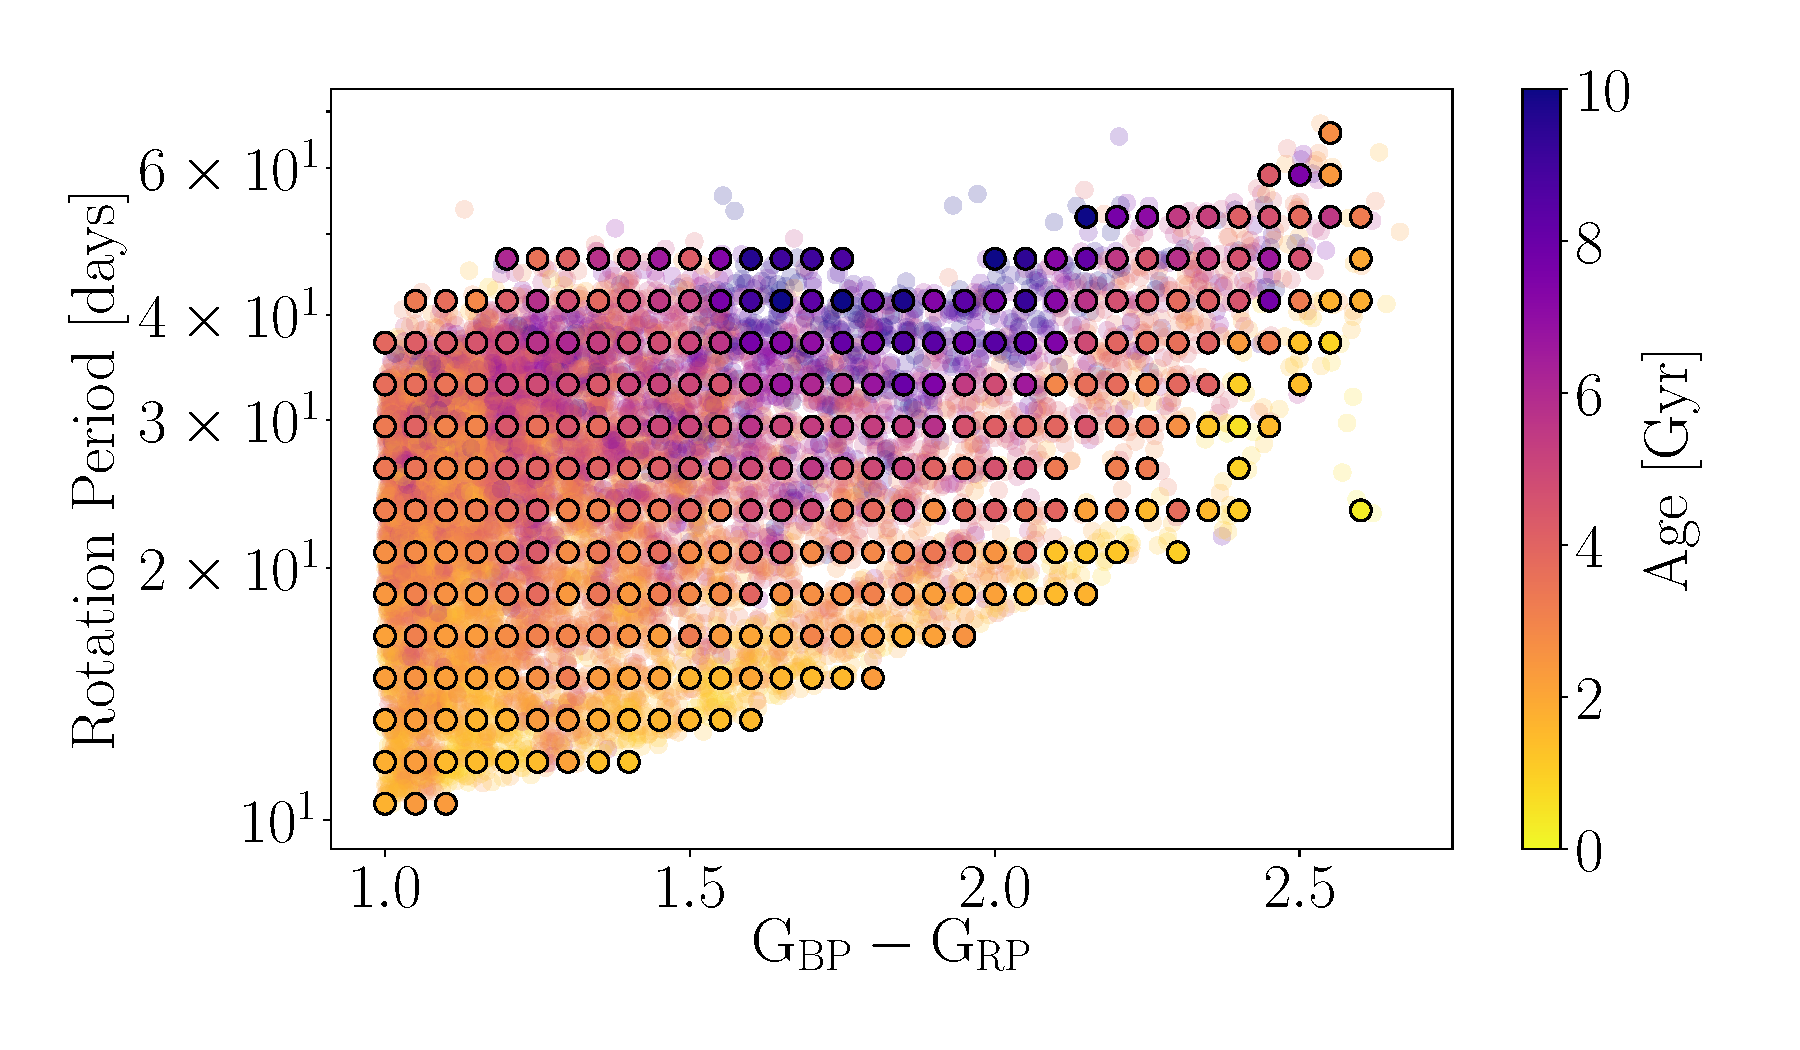
\includegraphics[width=1\textwidth]{grid_points}
\end{figure}

\begin{figure}
\caption{
}
  \centering 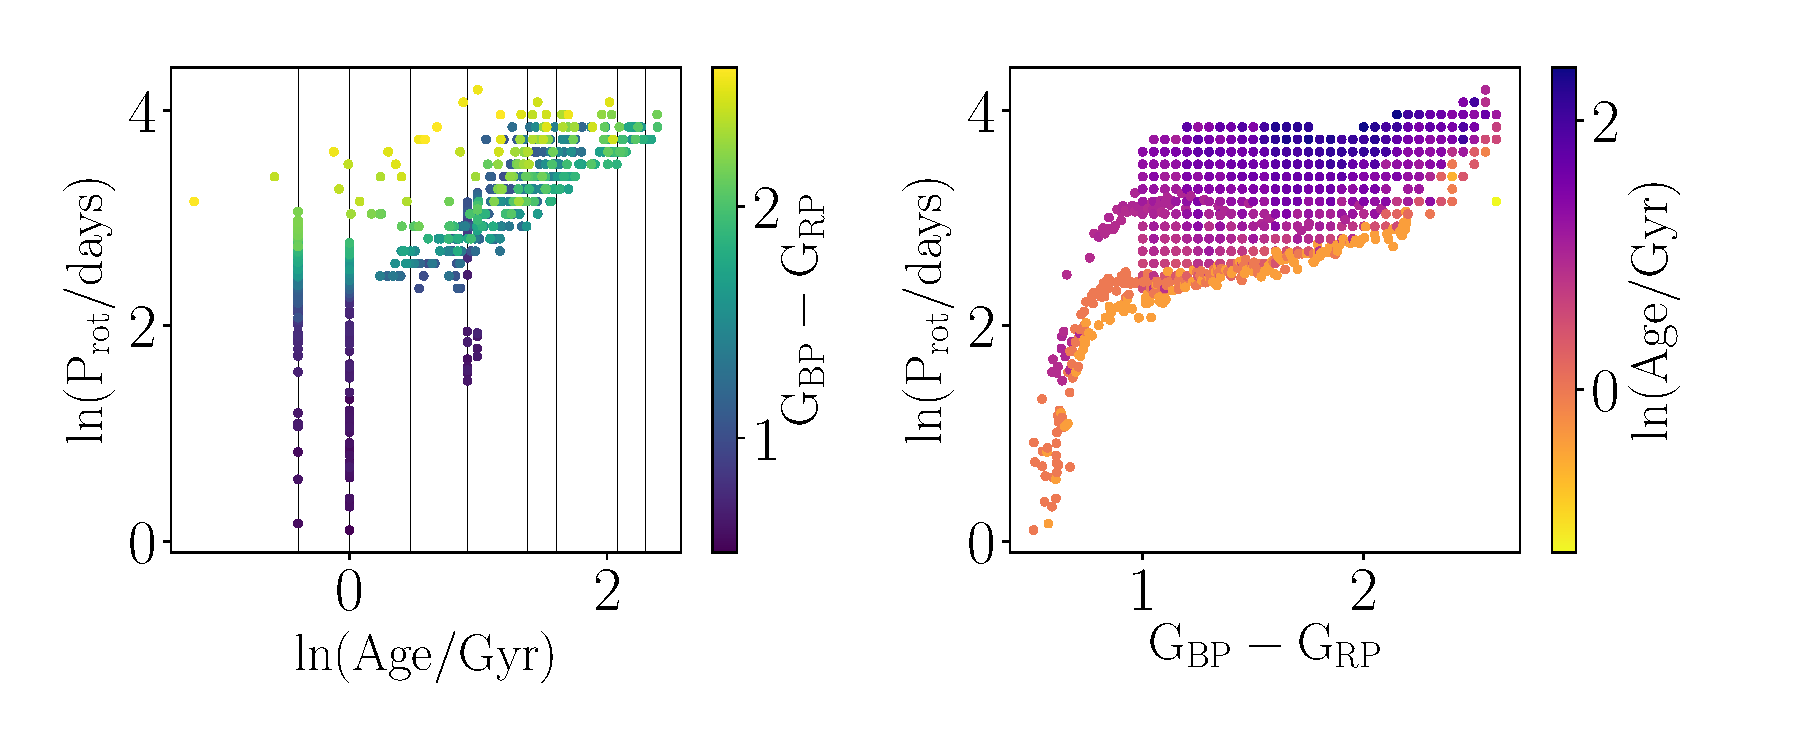
\includegraphics[width=1\textwidth]{gp_fit_data_multi-panel}
\end{figure}

\begin{figure}
\caption{
}
  \centering 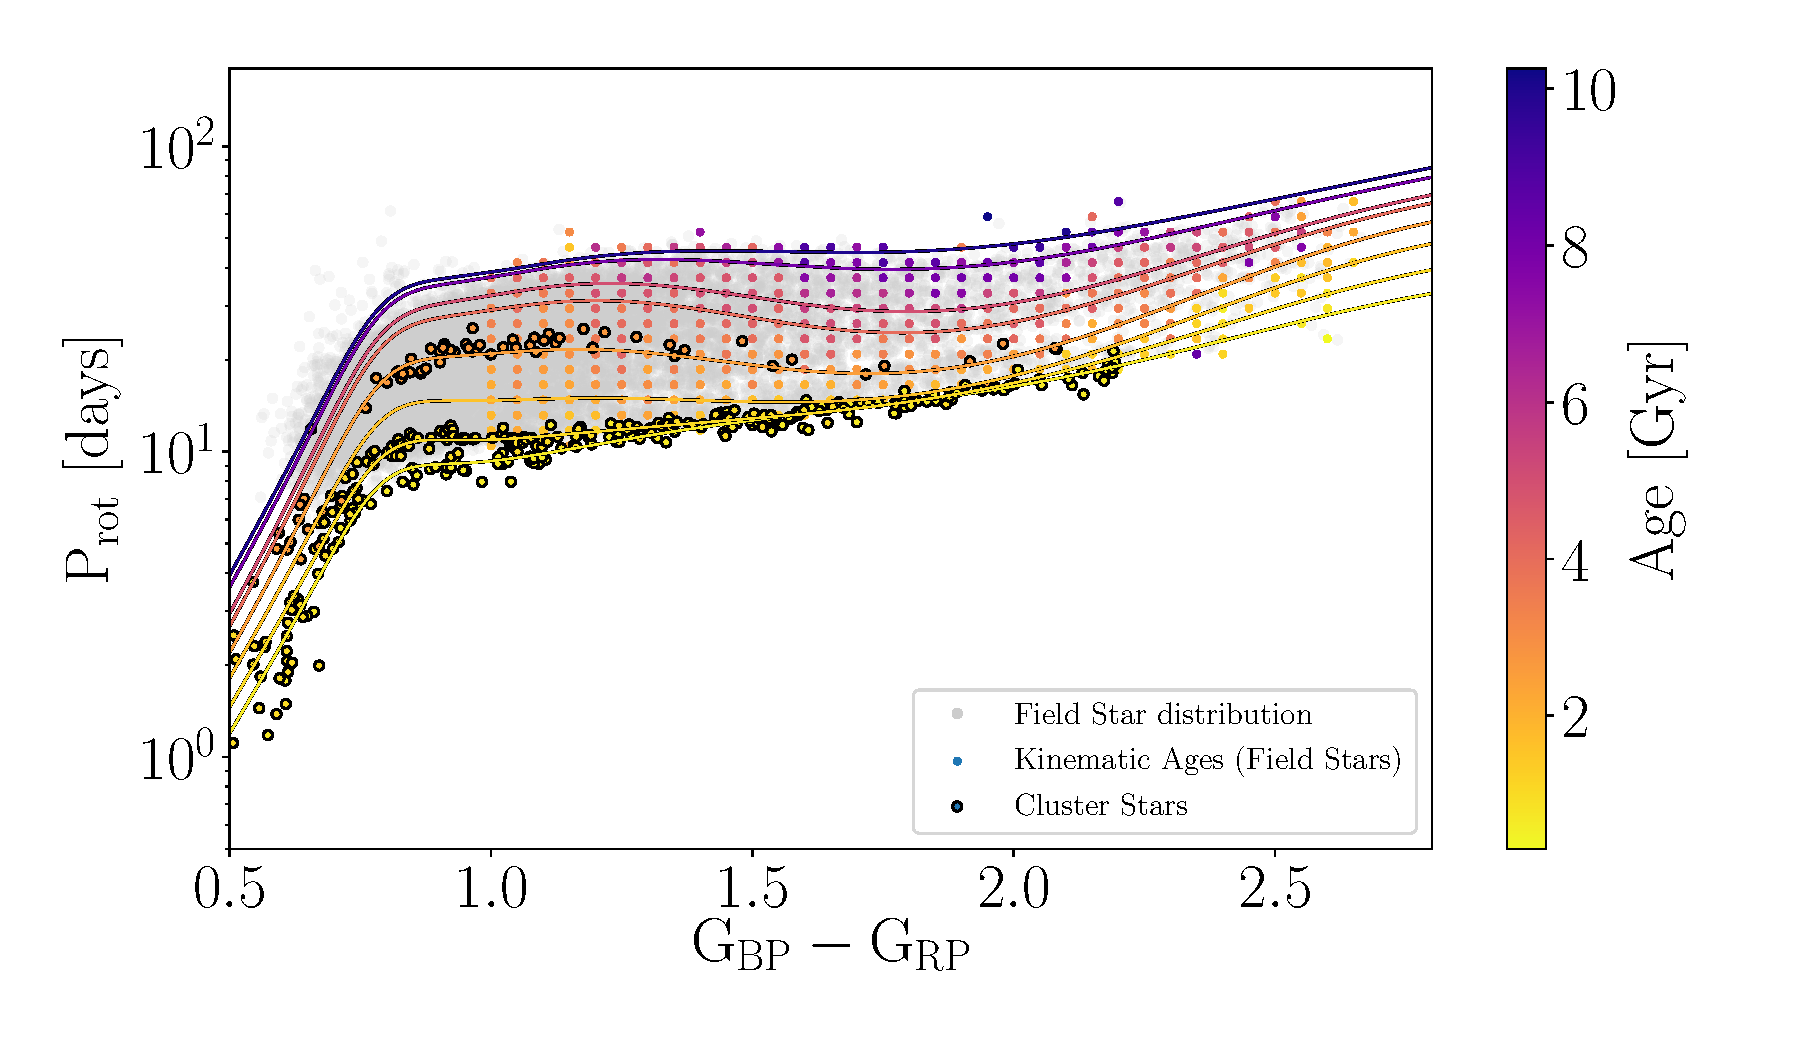
\includegraphics[width=1\textwidth]{gp_fit}
\end{figure}



\section{Discussion}


\section{Conclusion}

% Summarise motivation

% Summarise method

% Summarise results

% Summarise future


This work was partly developed at the 2019 KITP conference `Better stars,
better planets'.
Parts of this project are based on ideas explored at the Gaia sprints at the
Flatiron Institute in New York City, 2016 and MPIA, Heidelberg, 2017.
This work made use of the gaia-kepler.fun crossmatch database created by Megan
Bedell.

Some of the data presented in this paper were obtained from the Mikulski
Archive for Space Telescopes (MAST).
STScI is operated by the Association of Universities for Research in
Astronomy, Inc., under NASA contract NAS5-26555.
Support for MAST for non-HST data is provided by the NASA Office of Space
Science via grant NNX09AF08G and by other grants and contracts.
This paper includes data collected by the Kepler mission. Funding for the
\Kepler\ mission is provided by the NASA Science Mission directorate.

This work has made use of data from the European Space Agency (ESA) mission
{\it Gaia} (\url{https://www.cosmos.esa.int/gaia}), processed by the {\it
Gaia} Data Processing and Analysis Consortium (DPAC,
\url{https://www.cosmos.esa.int/web/gaia/dpac/consortium}).
Funding for the DPAC has been provided by national institutions, in particular
the institutions participating in the {\it Gaia} Multilateral Agreement.


\bibliography{aviary}{}
\bibliographystyle{aasjournal}

\end{document}
